\chapter{Payload System -- Tether Experiment}
\label{ch:payload_tether_experiment}

\section{Tether System and Experiment Description}
\label{sec:tether_sys_exp_desc}

The tether experiment is the primary payload of the LINKU mission. After SAT-BC is released from SAT-A and the SAT-B/SAT-C separation command is executed, SAT-B and SAT-C form a two-spacecraft tethered system connected by a non-conductive tether with a nominal length of \(100~\mathrm{m}\). The experiment is intended to observe the transition from the initially coupled SAT-B/SAT-C configuration to an extended tethered configuration in orbit.

The main objective of the experiment is to characterize the deployment behavior and subsequent tethered-system motion. The phenomena of interest include the relative separation between SAT-B and SAT-C, the release of the tether from its storage spool, tension build-up, possible slack/taut transitions, rebound or residual oscillations, and the evolution toward a gravity-gradient-influenced configuration. These effects are evaluated using the combined information from camera images, GNSS-derived relative motion, tether-tension measurements, and housekeeping telemetry.

The selected non-conductive tether configuration defines the experiment as a mechanical tether-dynamics mission. The data collected in orbit will be used for ground-based comparison with pre-flight tether-dynamics simulations, focusing on the observed deployment sequence, relative motion, and tension response. This understanding provides a technical basis for future tethered-spacecraft missions, including more complex concepts such as conductive or electrodynamic tether systems, where reliable deployment and tethered-system stability are also fundamental design problems.

\section{Separation and Tether Deployment Mechanism}
\label{sec:separation_tet_deploy_mech}

The SAT-B/SAT-C separation and tether deployment mechanism refers to the integrated subsystem responsible for separating SAT-B and SAT-C, releasing the tether stored in SAT-B, and providing the passive braking function required during deployment. In this section, this subsystem is referred to as the separation and deployment mechanism.

The LINKU mission sequence requires SAT-A to deploy the coupled SAT-BC unit before the internal separation between SAT-B and SAT-C is initiated. During this stage, SAT-BC refers to the integrated SAT-B and SAT-C configuration treated as a single coupled unit. The separation and deployment mechanism must then provide the initial relative motion between SAT-B and SAT-C, enable progressive tether release, and reduce the relative velocity near full tether extension. Due to the strict volume and mass constraints imposed by the non-standard SAT-BC geometry, the mechanism must be compact and efficiently integrated within the structure.

Several reference separation mechanisms were reviewed to identify design principles applicable to the SAT-B/SAT-C separation and tether deployment mechanism. The reviewed references include commercial separation and deployment systems, such as the Motorized Lightband MkII and CarboNIX NEO; the STARS-C tethered small-satellite mission, which used a spring-based separation and tether deployment mechanism; and other aerospace separation technologies, such as clamp-band systems based on explosive bolts~\cite{RocketLab2024MLB,Yamagiwa2017SpaceElevator,Cui2015SatelliteSeparation,Exolaunch2024CarboNIX}.

Although these references differ in scale, complexity, and release method, they show two design principles relevant to LINKU. First, stored mechanical energy, commonly provided by springs, is frequently used to generate the separation impulse. Second, a locking or restraint mechanism is required to keep the system constrained before activation. For LINKU, a spring-actuated concept with a simple locking and release mechanism was therefore selected as the preliminary solution, prioritizing compactness, simplicity, and compatibility with the SAT-BC geometry.

As described in the Satellite Separation and Tether Deployment Stage of Deliverable D4, the nominal relative separation velocity is in the range of \(0.5\)--\(1~\mathrm{m/s}\), with values below \(0.5~\mathrm{m/s}\) considered less favorable for reliable separation. For preliminary spring sizing, a conservative relative velocity of \(1.5~\mathrm{m/s}\) is considered to provide design margin with respect to the nominal separation condition and possible non-ideal effects. The following subsections present the spring sizing, passive braking estimate, tether container sizing, mechanical configuration, braking and storage configuration, and preliminary simulation of the separation and deployment mechanism.

\subsection{Separation Spring Sizing}
\label{sub:sep_spr_siz}

The separation spring system must provide the initial impulse required to separate SAT-B and SAT-C while satisfying the spatial constraints imposed by the SAT-B internal configuration. In the current preliminary design, the maximum allowable spring height is 43 mm, which is limited by the available volume inside SAT-B. Based on the deployment analysis presented in Deliverable D4, the nominal operational range for the relative separation velocity is approximately 0.5--1 m/s. For preliminary spring sizing, a conservative relative velocity of 1.5 m/s is considered to provide design margin with respect to the nominal operational range and to account for idealized assumptions and possible losses during the release process.

The required equivalent stiffness of the spring system is estimated by equating the elastic energy stored in the compressed springs to the kinetic energy acquired by SAT-B and SAT-C after release:

\begin{equation}
\frac{1}{2} K_{eq} x^2 =
\frac{1}{2} m_B v_B^2 +
\frac{1}{2} m_C v_C^2 ,
\label{eq:spring_energy_balance}
\end{equation}

where \(K_{eq}\) is the equivalent stiffness of the springs in parallel, \(x\) is the spring compression, \(m_B\) and \(m_C\) are the masses of SAT-B and SAT-C, and \(v_B\) and \(v_C\) are their velocities after separation, respectively.

The estimated masses of SAT-B and SAT-C are approximately \(m_B = 5~\mathrm{kg}\) and \(m_C = 0.5~\mathrm{kg}\). Since both satellites are initially at rest with respect to each other, conservation of linear momentum gives

\begin{equation}
m_B v_B + m_C v_C = 0 .
\label{eq:momentum_balance_satbc}
\end{equation}

Using the mass ratio between SAT-B and SAT-C, Eq.~\eqref{eq:momentum_balance_satbc} becomes

\begin{equation}
v_C = -10v_B .
\label{eq:velocity_mass_ratio}
\end{equation}

The relative separation velocity is defined as

\begin{equation}
v_{rel} = v_C - v_B .
\label{eq:relative_velocity_definition}
\end{equation}

For the sizing case \(v_{rel}=1.5~\mathrm{m/s}\), Eqs.~\eqref{eq:velocity_mass_ratio} and \eqref{eq:relative_velocity_definition} give

\begin{equation}
v_C = 1.364~\mathrm{m/s},
\qquad
v_B = -0.136~\mathrm{m/s}.
\label{eq:satbc_velocity_values}
\end{equation}

Substituting these values into Eq.~\eqref{eq:spring_energy_balance}, the required stored elastic energy is obtained as

\begin{equation}
\frac{1}{2} K_{eq} x^2 =
\frac{1}{2}(5)(0.136)^2 +
\frac{1}{2}(0.5)(1.364)^2
\approx 0.5105~\mathrm{J}.
\label{eq:required_elastic_energy}
\end{equation}

Therefore,

\begin{equation}
K_{eq}x^2 \approx 1.021~\mathrm{N\,m}.
\label{eq:keq_x2_requirement}
\end{equation}

If the mechanism uses \(n_s\) identical springs arranged in parallel, the equivalent stiffness is

\begin{equation}
K_{eq} = n_s K_s ,
\label{eq:equivalent_stiffness_parallel}
\end{equation}

where \(K_s\) is the stiffness of each individual spring. The spring sizing condition can therefore be written as

\begin{equation}
n_s K_s x^2 \approx 1.021~\mathrm{N\,m}.
\label{eq:spring_array_sizing_condition}
\end{equation}

This result defines the minimum elastic energy that the spring array must provide for the conservative sizing case. The final spring selection must also account for available compression length, mechanical stops, release losses, friction, locking/release tolerances, and compatibility between the resulting separation velocity and the tether braking requirement.

\subsection{Braking and Terminal Relative Velocity}
\label{sub:braking_terminal_velocity}

The SAT-B/SAT-C separation and tether deployment mechanism must reduce the relative velocity of the satellites before the tether reaches its full extension. If the relative velocity generated during the initial separation were maintained until the tether reaches its nominal length of 100 m, a high tension peak and a rebound event could occur.

The deployment analysis presented in Deliverable D4 indicates that the terminal relative velocity should be reduced to \(0.1~\mathrm{m/s}\) or lower near full tether extension. For preliminary sizing, the braking system is conservatively assumed to dissipate the full kinetic energy associated with the initial relative separation velocity. This assumption provides margin with respect to the terminal velocity requirement.

From the spring sizing analysis in Section~\ref{sub:sep_spr_siz}, the elastic energy required for the conservative separation case is approximately \(0.5105~\mathrm{J}\). Assuming that this energy must be dissipated by the tether braking system, the required braking work is

\begin{equation}
W_b \approx 0.5105~\mathrm{J}.
\label{eq:braking_work_full_stop}
\end{equation}

If the braking force is assumed to act approximately over the full tether deployment length, the average dissipative force can be estimated as

\begin{equation}
W_b = F_f d,
\label{eq:braking_work_friction}
\end{equation}

where \(F_f\) is the average friction force and \(d\) is the deployment distance. For a nominal tether length of \(d=100~\mathrm{m}\),

\begin{equation}
F_f =
\frac{W_b}{d}
=
\frac{0.5105}{100}
\approx
5.1\times10^{-3}~\mathrm{N}
=
5.1~\mathrm{mN}.
\label{eq:average_friction_force_value}
\end{equation}

If the braking target is taken as \(v_{\mathrm{rel},f}=0.1~\mathrm{m/s}\) instead of a full stop, the required dissipated energy decreases only slightly, from approximately \(0.5105~\mathrm{J}\) to \(0.509~\mathrm{J}\). Therefore, the same average dissipative force of approximately \(5.1~\mathrm{mN}\) is retained as the preliminary braking requirement.

This value should be interpreted as a first-order estimate. The actual braking force will depend on the tether routing, contact geometry, friction coefficient, spool configuration, and deployment dynamics. The braking performance must therefore be verified through dedicated ground tests and updated simulations.

\subsection{Tether Container}
\label{sub:tether_container}

The tether must be stored inside SAT-B in a controlled configuration prior to deployment. The container is intended to protect the tether, reduce the risk of entanglement with internal structures, and maintain an organized release path during the SAT-B/SAT-C separation process. This is necessary to support progressive tether deployment and to reduce the probability of knots or uncontrolled release.

The minimum storage volume can be estimated from the geometric volume of the tether. As a preliminary reference for sizing, the calculation assumes the diameter of the Kevlar tether candidate considered in the current mechanical concept. Approximating the tether as a cylinder, its volume is given by

\begin{equation}
V_t = \pi r_t^2 L_t ,
\label{eq:tether_volume}
\end{equation}

where \(V_t\) is the tether volume, \(r_t\) is the tether radius, and \(L_t\) is the tether length. For a nominal tether length of \(L_t = 100~\mathrm{m} = 10000~\mathrm{cm}\) and a reference tether radius of \(r_t = 0.05~\mathrm{cm}\), Eq.~\eqref{eq:tether_volume} gives

\begin{equation}
V_t =
\pi (0.05)^2(10000)
\approx 78.5~\mathrm{cm^3}.
\label{eq:tether_volume_value}
\end{equation}

Additional volume must be allocated for the spool, packing inefficiencies, internal clearances, and supporting elements required to guide the tether during release. In this preliminary design, a margin of approximately 27\% is applied to the estimated tether volume. Therefore, the minimum allocated container volume is

\begin{equation}
V_{\mathrm{cont,min}}
=
1.27 V_t
\approx
1.27(78.5)
\approx
100~\mathrm{cm^3}.
\label{eq:minimum_container_volume}
\end{equation}

This value defines the preliminary volume requirement for the tether container.

\subsection{Preliminary Mechanical Configuration}
\label{sub:preliminary_mechanical_configuration}

Once the functional requirements and spring sizing condition have been established, the preliminary mechanical configuration of the SAT-B/SAT-C separation mechanism can be defined. The mechanism has undergone several design iterations to improve compactness, alignment, manufacturability, and reliability within the available SAT-B volume.

The current preliminary configuration is based on four commercial compression springs arranged in parallel, with an equivalent stiffness of \(K_{eq}=5200~\mathrm{N/m}\). This value is used to verify whether the mechanism can provide the required separation energy established in Eq.~\eqref{eq:spring_array_sizing_condition}. According to the manufacturer specifications, the selected springs have a recommended maximum deformation of \(17.86~\mathrm{mm}\).

Using the spring sizing condition,

\begin{equation}
K_{eq}x^2 = 1.021~\mathrm{N\,m},
\label{eq:mechanical_config_spring_condition}
\end{equation}

and substituting \(K_{eq}=5200~\mathrm{N/m}\), the required spring compression is

\begin{equation}
x =
\sqrt{\frac{1.021}{5200}}
\approx
0.0140~\mathrm{m}
=
14~\mathrm{mm}.
\label{eq:required_spring_compression}
\end{equation}

Therefore, a minimum spring compression of approximately \(14~\mathrm{mm}\) is required to satisfy the conservative separation energy condition. In the current configuration, a compression of \(15.5~\mathrm{mm}\) is used to provide margin with respect to frictional losses, release tolerances, and other non-ideal effects not included in the analytical estimate. This value remains below the recommended maximum spring deformation of \(17.86~\mathrm{mm}\).

With the spring model and compression value defined, the separation mechanism was configured to fit within the SAT-B/SAT-C geometry. An initial concept using five springs was considered to improve load distribution; however, the geometry of SAT-B favors an even number of springs, simplifying the mechanical layout and assembly. For this reason, the current design uses four compression springs arranged around the central axis of the mechanism.

Each spring is housed within a spring enclosure and guided by corresponding ejection guide rails. These rails constrain the motion of the ejection plate, ensuring that SAT-C is pushed along the common axis between SAT-B and SAT-C. The separation mechanism is also arranged around the tether container, allowing the available internal volume of SAT-B to be used efficiently and enabling tether release immediately after SAT-C separation. Figure~\ref{fig:closed_separation_system} shows the mechanism with the compression springs in their compressed state.

\begin{figure}[htbp]
    \centering
    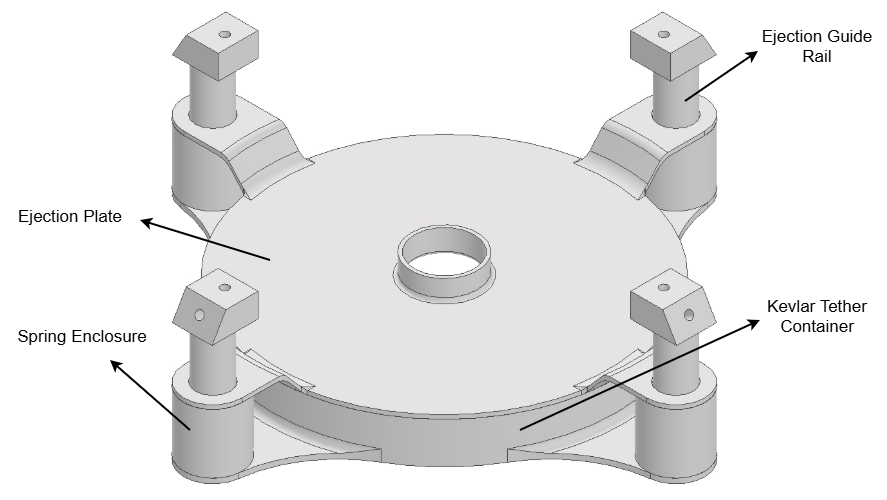
\includegraphics[width=0.88\linewidth]{PUCP_pictures/Closed Separation System.png}
    \caption{Closed configuration of the SAT-B/SAT-C separation mechanism.}
    \label{fig:closed_separation_system}
\end{figure}

The ejection guide rails are attached to the SAT-B structure to provide alignment and stiffness during separation. The force generated by the springs is transmitted through the ejection plate pushers to the ejection plate, which is the component that transfers the impulse to SAT-C. Figure~\ref{fig:open_separation_system} shows the mechanism after release, when the springs have expanded and the ejection plate has moved along the guide rails. Mechanical stops are included to keep the ejection plate inside SAT-B and prevent it from being expelled together with SAT-C.

\begin{figure}[htbp]
    \centering
    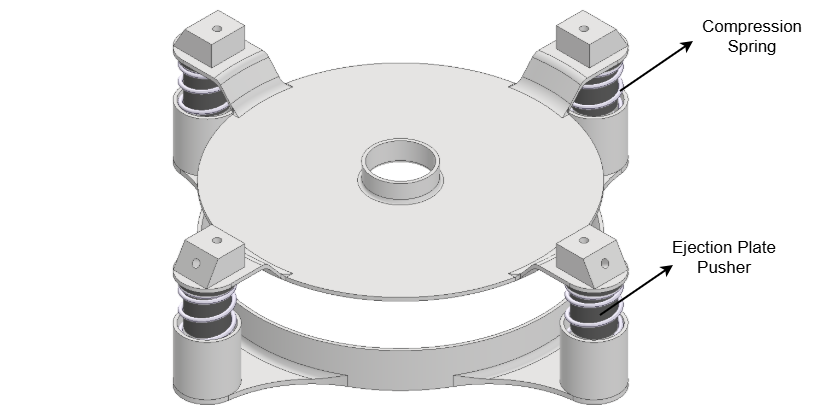
\includegraphics[width=0.9\linewidth]{PUCP_pictures/Open Separation System.png}
    \caption{Open configuration of the SAT-B/SAT-C separation mechanism after spring release.}
    \label{fig:open_separation_system}
\end{figure}

The ejection plate includes a central cylindrical guide that fits into a corresponding hole in SAT-C. This guide helps maintain the relative alignment between SAT-C and the separation mechanism before release. As a result, the initial separation motion is constrained primarily along the common axial direction of the two satellites.

The mechanism also incorporates a locking system to keep the springs compressed until the separation command is issued. In the current prototype, the locking concept is based on a nylon restraint thread routed through SAT-C, with its ends secured to retention pulleys mounted on the upper face of SAT-B. In this configuration, the nylon thread acts as a restraint element that prevents SAT-C and the ejection plate from moving under the stored spring force.

A nichrome heating element is proposed as the release actuator. When activated, the heating element melts the nylon restraint thread, removes the constraint, and allows the elastic energy stored in the springs to be released. Figure~\ref{fig:satc_locking_system} shows the locking system integrated into the SAT-C structure. The thread is routed through guides located in the outer regions of the SAT-C base, while the thermal cutting module is located near the central region where the thread passes through SAT-C.

\begin{figure}[htbp]
    \centering
    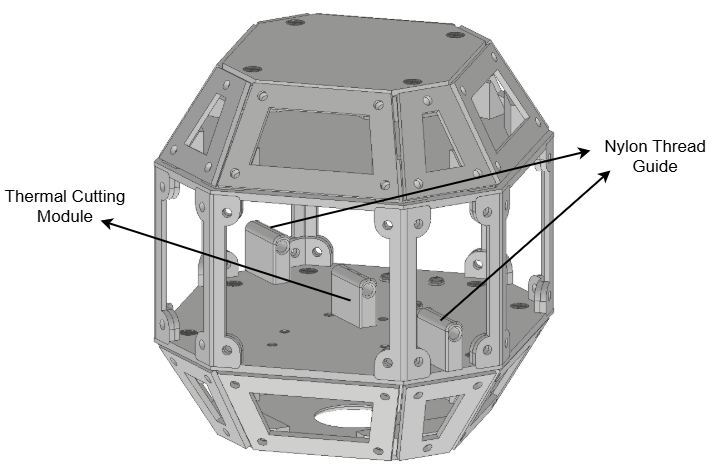
\includegraphics[width=0.8\linewidth]{PUCP_pictures/SATC_Structure_Locking_System.png}
    \caption{Locking system integrated into the SAT-C structure.}
    \label{fig:satc_locking_system}
\end{figure}

Figure~\ref{fig:locking_system_satb} shows the integration of the separation mechanism and SAT-C on the upper section of SAT-B. The base of the separation mechanism is fastened to the upper octagonal base of SAT-B using bolts located near the ejection guide rails. The upper ends of the guide rails are attached to the top plate of SAT-B, providing additional support and maintaining the separation trajectory. The retention pulleys mounted on the upper surface of SAT-B secure the nylon restraint thread and keep it under tension until activation.

\begin{figure}[htbp]
    \centering
    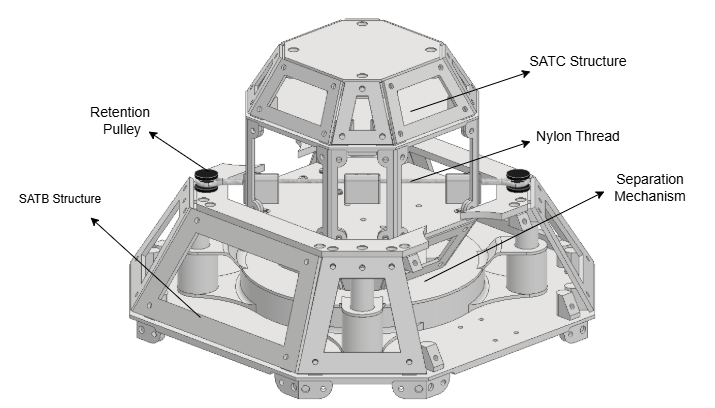
\includegraphics[width=1\linewidth]{PUCP_pictures/Locking System Integrated into the SATB.png}
    \caption{Locking system integrated into the SAT-B structure.}
    \label{fig:locking_system_satb}
\end{figure}

The present configuration represents the most recent preliminary design of the SAT-B/SAT-C separation mechanism. Based on the analytical sizing performed in Section~\ref{sub:sep_spr_siz}, the selected spring arrangement and compression level provide the required separation energy with additional margin. The locking and thermal release concept allows the springs to remain compressed before deployment and to release the stored elastic energy when the separation command is issued. Nevertheless, alternative locking and release configurations are still being evaluated as part of the design maturation process toward the PDR stage.

At this stage, the simulation effort focuses on validating the dynamic response of the current mechanical configuration, particularly the release of the stored spring energy and the resulting motion of SAT-C. This validation is necessary because the analytical sizing does not capture all contact interactions, alignment constraints, and non-ideal effects. The following section presents the simulation approach used to evaluate the consistency of the mechanism performance with the intended separation conditions.

\subsection{Separation System Simulation and Validation}
\label{sub:separation_system_simulation}

A transient structural simulation was performed in ANSYS to evaluate the dynamic response of the current SAT-B/SAT-C separation mechanism. The objective of the simulation was to verify whether the release of the elastic energy stored in the springs produces a SAT-C separation velocity compatible with the preliminary deployment requirements.

The simulation model was derived from the preliminary mechanical configuration described in Section~\ref{sub:preliminary_mechanical_configuration}. To reduce computational cost, the CAD model was simplified while preserving the main components involved in the separation process. The simplified model includes the compression springs, the ejection plate, the ejection guide rails, the spring enclosures, and the ejection plate pushers. SAT-C was represented as a single solid body with a mass of \(0.5~\mathrm{kg}\), consistent with the value used in the analytical spring sizing presented in Section~\ref{sub:sep_spr_siz}.

In this preliminary simulation, SAT-B was assumed to be fixed. Therefore, the complete two-body separation problem, in which SAT-B and SAT-C move in opposite directions, was not modeled. Instead, the octagonal base of SAT-B was used as a fixed reference, and the velocity of SAT-C was interpreted as the relative separation velocity with respect to SAT-B. The simplified 3D model used in the simulation is shown in Figure~\ref{fig:ansys_separation_model}.

\begin{figure}[htbp]
    \centering
    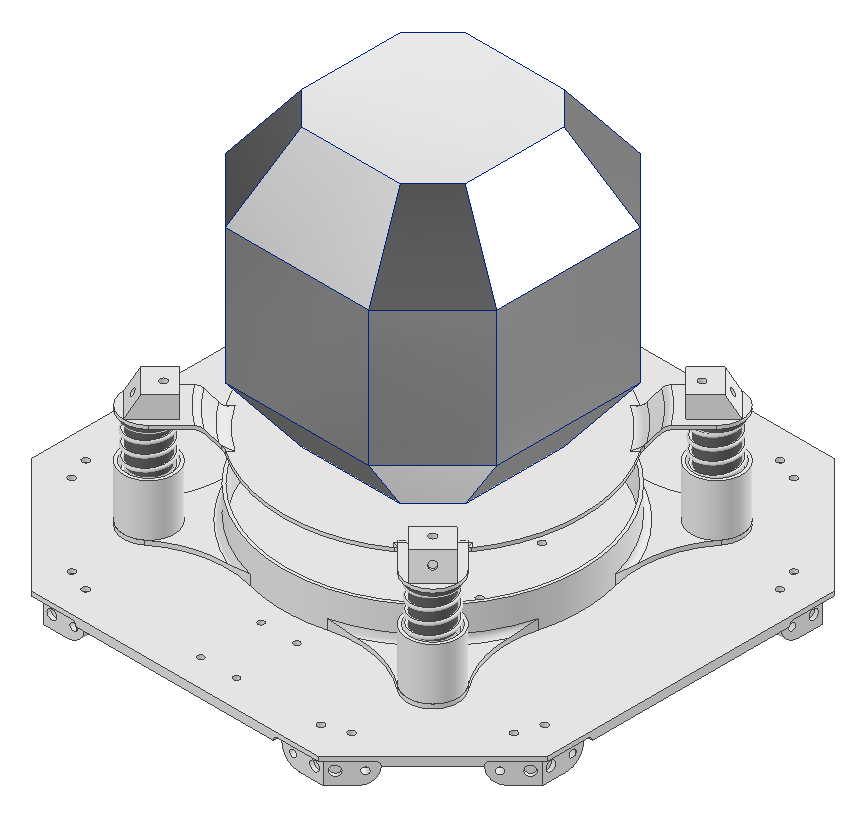
\includegraphics[width=0.7\linewidth]{PUCP_pictures/3D Model of the Separation Mechanism for ANSYS Simulation.png}
    \caption{Simplified 3D model of the SAT-B/SAT-C separation mechanism used for the transient structural simulation.}
    \label{fig:ansys_separation_model}
\end{figure}

The material properties were assigned according to the preliminary component definitions. Stainless steel was used for the compression springs, following the manufacturer specifications, while aluminum was assigned to SAT-C and to the remaining structural components included in the model.

The mechanical interactions were defined using joints and contacts. Cylindrical joints were used to constrain the motion of SAT-C and the ejection plate along the common separation axis. This constraint allows axial translation and rotation about the same axis, while preventing lateral motion during the simulated release. Figure~\ref{fig:cylindrical_joint_satc} shows the cylindrical joint used to constrain SAT-C with respect to the separation mechanism.

\begin{figure}[htbp]
    \centering
    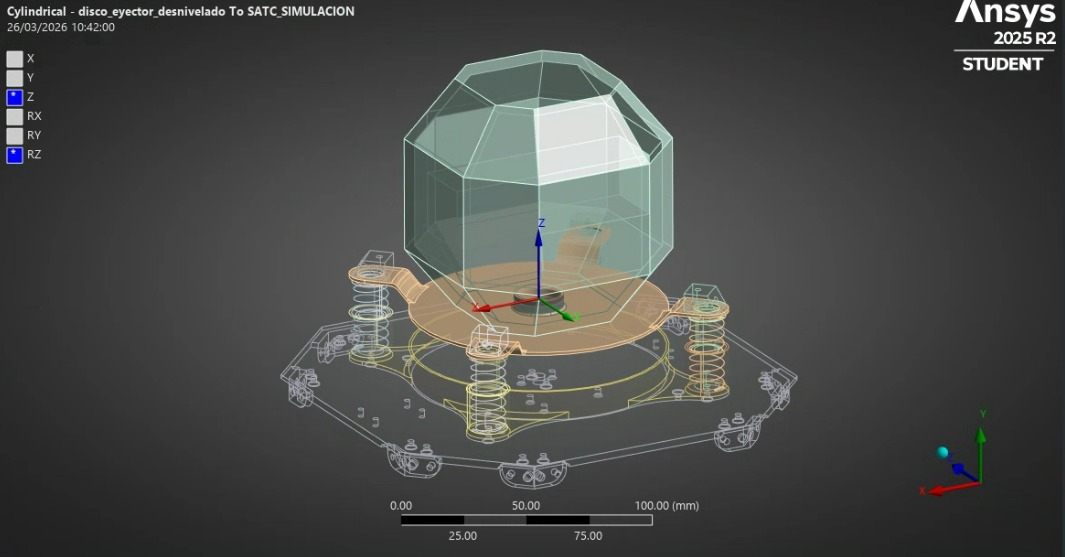
\includegraphics[width=0.8\linewidth]{PUCP_pictures/“Cylindrical” Motion Constraint Between the Separation Mechanism and the SATC.jpeg}
    \caption{Cylindrical joint used to constrain the SAT-C motion along the separation axis.}
    \label{fig:cylindrical_joint_satc}
\end{figure}

Fixed joints were used between the compression springs, the spring enclosures, and the ejection plate pushers. This simplification keeps the springs in contact with the corresponding components during the simulated compression and release process. Although these elements are not permanently bonded in the physical assembly, the assumption is acceptable for this preliminary model because the springs remain compressed and in continuous contact during the release event. Figure~\ref{fig:fixed_joint_springs} shows the fixed joint definition used for the spring interfaces.

\begin{figure}[htbp]
    \centering
    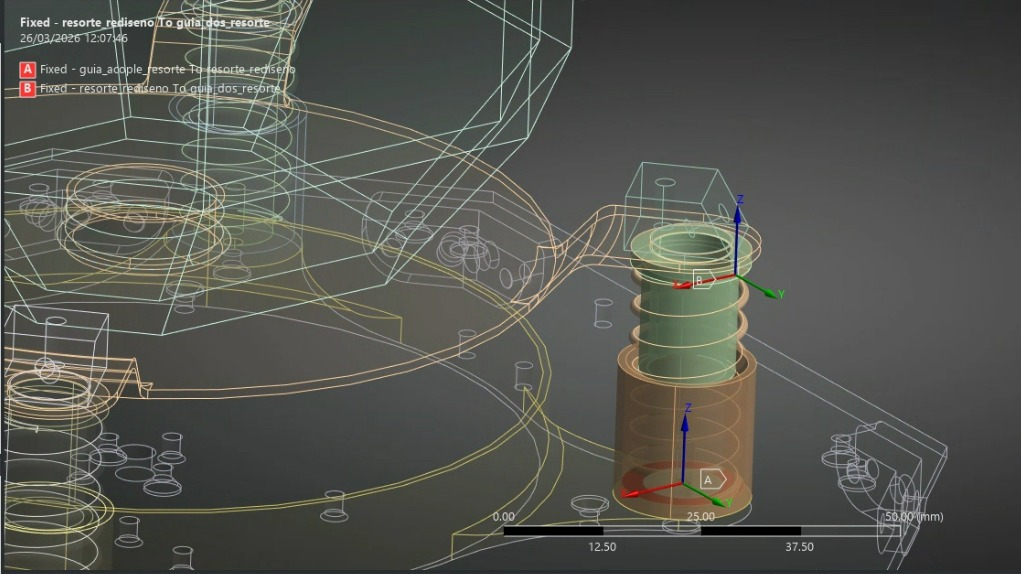
\includegraphics[width=0.8\linewidth]{PUCP_pictures/Fixed-type joint for the springs with the spring enclosure and the ejection plate pusher..jpeg}
    \caption{Fixed joint definition between the springs, spring enclosures, and ejection plate pushers.}
    \label{fig:fixed_joint_springs}
\end{figure}

Frictionless contacts were used at the main interaction surfaces. In particular, a frictionless contact was defined between the upper face of the ejection plate and the lower face of SAT-C, allowing the spring force to be transferred to SAT-C while neglecting friction losses at this stage. The same contact approach was applied to the interaction between the ejection plate arms and the guide rail stops. The contact between the ejection plate and SAT-C is shown in Figure~\ref{fig:frictionless_contact_plate_satc}.

\begin{figure}[htbp]
    \centering
    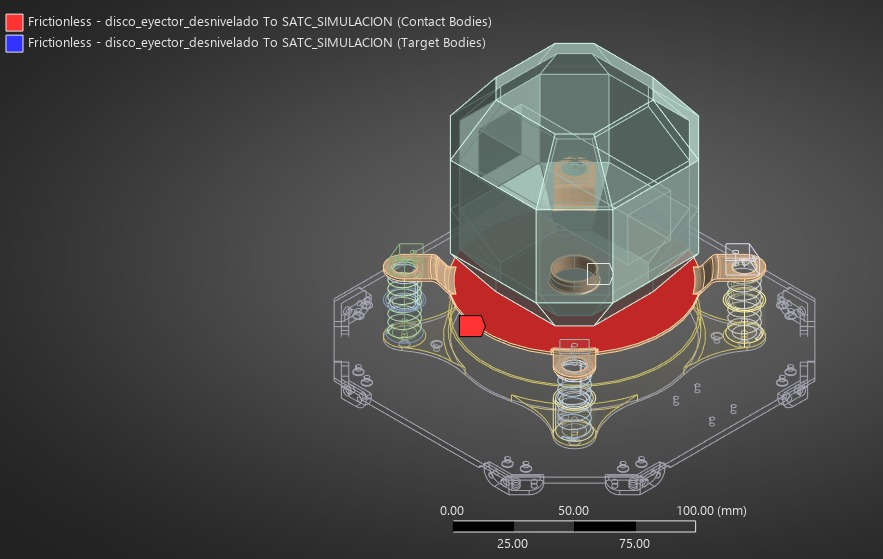
\includegraphics[width=0.8\linewidth]{PUCP_pictures/Contact type “Frictionless” between the Ejection Plate and the lower base of the SATC.jpeg}
    \caption{Frictionless contact between the ejection plate and the lower face of SAT-C.}
    \label{fig:frictionless_contact_plate_satc}
\end{figure}

A global mesh size of \(2~\mathrm{mm}\) was used for the assembly. A finer mesh was applied to the spring regions because of their smaller geometric features, with a wire thickness of approximately \(1~\mathrm{mm}\). Under these conditions, the mesh quality reported by ANSYS was approximately \(76\%\), as shown in Figure~\ref{fig:mesh_quality_ansys}.

\begin{figure}[htbp]
    \centering
    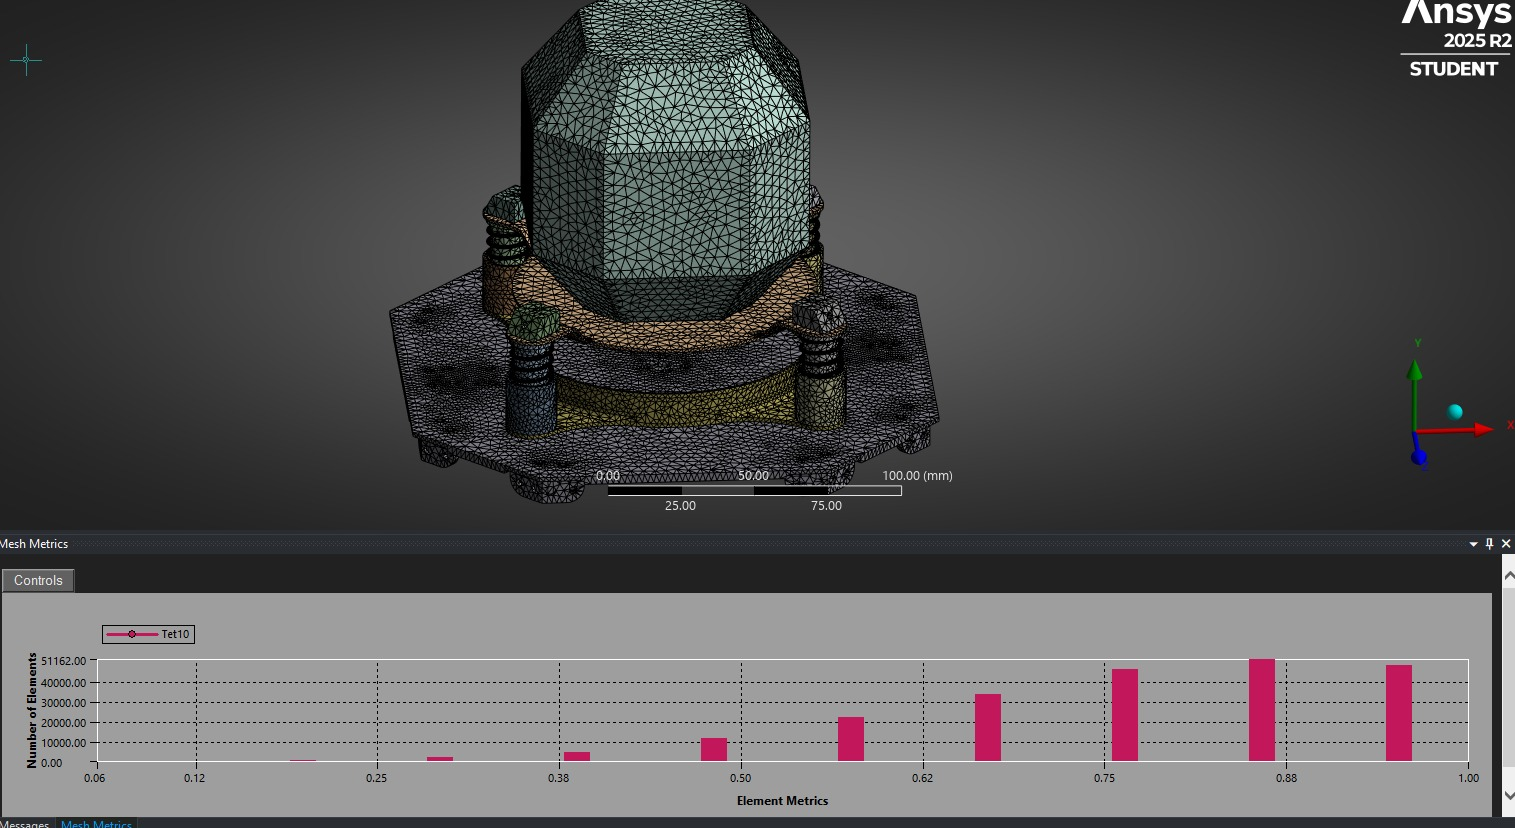
\includegraphics[width=0.8\linewidth]{PUCP_pictures/Finite element mesh quality for the simulation..jpeg}
    \caption{Finite element mesh quality reported for the transient structural simulation.}
    \label{fig:mesh_quality_ansys}
\end{figure}

The boundary conditions were defined to reproduce the compression and release sequence. First, the lower face of the SAT-B base was fixed, preventing translations and rotations of the reference structure. Second, a prescribed displacement was applied to SAT-C along the negative \(Y\)-axis to compress the springs through the ejection plate. Once a spring compression of \(15.5~\mathrm{mm}\) was reached, the prescribed displacement condition was removed, allowing the springs to release their stored elastic energy. The boundary conditions used in the simulation are shown in Figure~\ref{fig:boundary_conditions_ansys}.

\begin{figure}[htbp]
    \centering
    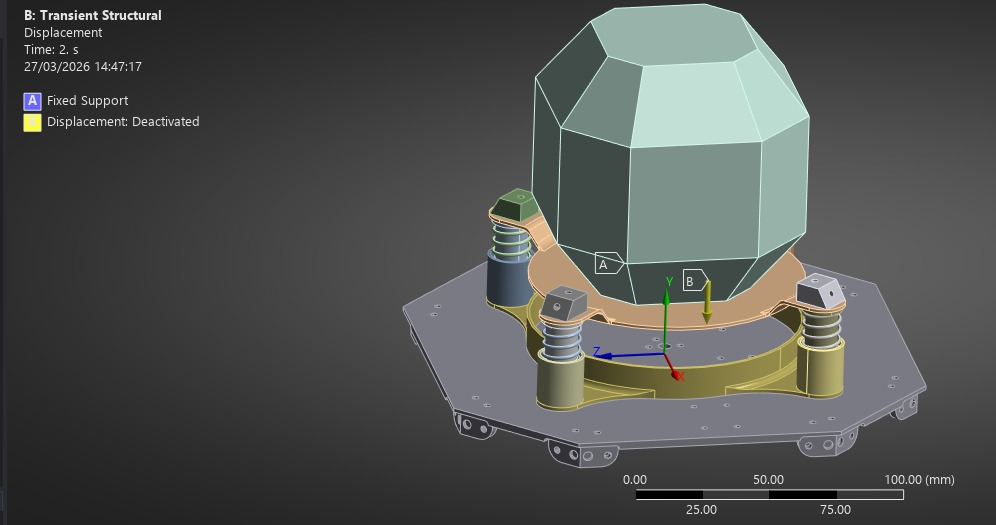
\includegraphics[width=0.8\linewidth]{PUCP_pictures/Boundary conditions of the simulation.jpeg}
    \caption{Boundary conditions used for the compression and release simulation.}
    \label{fig:boundary_conditions_ansys}
\end{figure}

The simulation was divided into two stages. During the first second, a prescribed motion was applied to bring the mechanism to its compressed configuration. The velocity observed during this interval, approximately \(0.3~\mathrm{m/s}\), corresponds to the imposed compression step and should not be interpreted as the separation velocity. During the second stage, the imposed displacement condition was removed, allowing the springs to expand and transfer momentum to the ejection plate and subsequently to SAT-C. The total simulated time was \(2~\mathrm{s}\), including the compression and release phases.

The analytical sizing presented in Section~\ref{sub:sep_spr_siz} considered a conservative relative separation velocity of \(1.5~\mathrm{m/s}\). The transient simulation produced a SAT-C separation velocity of approximately \(1.24~\mathrm{m/s}\), as shown in Figure~\ref{fig:separation_velocity_result}. This value is above the nominal lower bound of \(0.5~\mathrm{m/s}\), remains below the conservative sizing case of \(1.5~\mathrm{m/s}\), and is therefore compatible with the preliminary separation objective.

\begin{figure}[htbp]
    \centering
    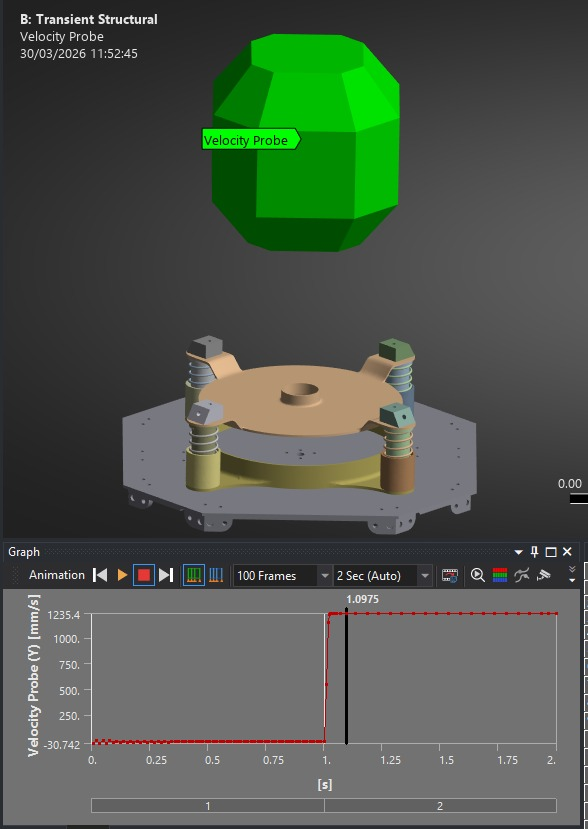
\includegraphics[width=0.52\linewidth]{PUCP_pictures/Simulation results of the separation of satellites SATB and SATC.jpeg}
    \caption{Simulation result for the SAT-C separation velocity during the release stage.}
    \label{fig:separation_velocity_result}
\end{figure}

The difference between the analytical value and the simulated velocity is expected, since the simulation includes geometric constraints, contacts, mechanical stops, and other non-ideal interactions that are not represented in the simplified energy balance. The result indicates that the current spring-actuated mechanism can provide a separation velocity compatible with the preliminary deployment objective. Further simulations and ground tests are still required to assess sensitivity to friction, alignment errors, release timing, and locking mechanism behavior.

\subsection{Tether Braking and Storage Configuration}
\label{sub:tether_braking_storage}

This subsection presents the preliminary physical configuration used to implement the passive tether braking function and the tether storage volume within SAT-B. The configuration is based on the average dissipative force estimated in Section~\ref{sub:braking_terminal_velocity} and on the minimum container volume defined in Section~\ref{sub:tether_container}.

As discussed in Section~\ref{sub:braking_terminal_velocity}, the tether deployment system requires a passive braking function to reduce the terminal relative velocity of SAT-B and SAT-C near full tether extension. The preliminary estimate indicated that an average dissipative force of approximately \(5.1~\mathrm{mN}\) is required over the nominal tether deployment length.

Because the required braking force is relatively low, a passive friction-based configuration was selected for the preliminary design. Active alternatives, such as mechanisms capable of adjusting the diameter of the tether exit hole, were considered but were not retained at this stage because their added complexity is not justified by the estimated friction level. The passive concept consists of a central conical spool with an internal orifice through which the tether passes before being wound around the spool. The spool is positioned on the octagonal base of SAT-B, inside the tether container and directly below the ejection plate.

The braking principle is based on friction generated at the tether contact points during deployment. These contact points include the interaction between the tether and the spool, as well as the interaction between the tether and the exit orifice of the ejection plate. The corresponding friction forces, denoted as \(F_{f,1}\) and \(F_{f,2}\), are illustrated in Figure~\ref{fig:tether_braking_storage_section}.

\begin{figure}[htbp]
    \centering
    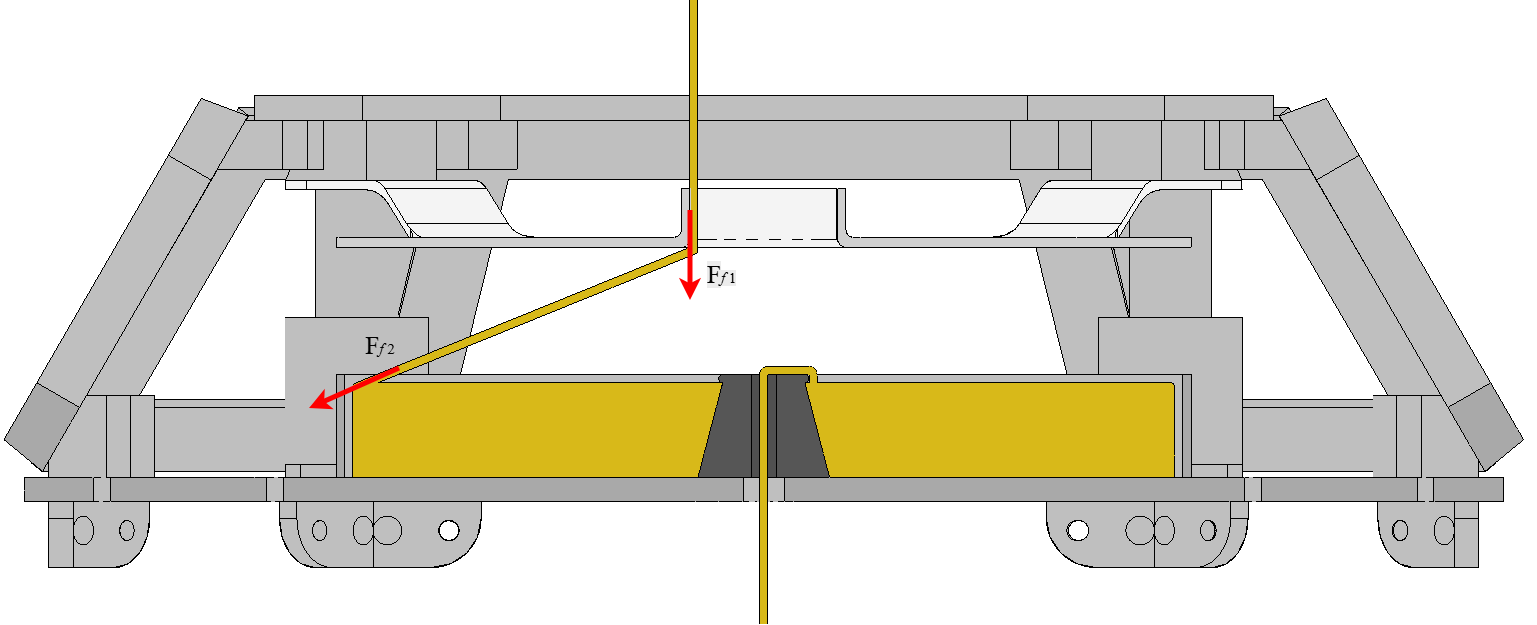
\includegraphics[width=1\linewidth]{PUCP_pictures/Cross-sectional view of the Kevlar thread deceleration and containment system.png}
    \caption{Cross-sectional view of the tether braking and storage configuration.}
    \label{fig:tether_braking_storage_section}
\end{figure}

At this stage, the exact friction produced at the contact points has not yet been quantified. Therefore, the proposed configuration must be evaluated through simulation and prototyping to determine whether it can generate the required average dissipative force of approximately \(5.1~\mathrm{mN}\). A dedicated test bench is planned to experimentally measure the friction produced by the selected tether routing and contact configuration.

The container geometry was defined to provide at least \(100~\mathrm{cm^3}\) of storage volume, as established in Section~\ref{sub:tether_container}. To satisfy this requirement while remaining compatible with the SAT-B internal structure, the design maximizes the available area on the octagonal base and minimizes the container height.

The container height is constrained by the accommodation of the SAT-B/SAT-C system within SAT-A and by the presence of other internal subsystems and mechanisms. For this reason, a height below \(15~\mathrm{mm}\) was targeted. The current preliminary container has a cylindrical geometry with a diameter of \(102~\mathrm{mm}\) and a height of \(12.5~\mathrm{mm}\). Inside the container, the tether is wound around a central conical spool. The spool has a larger base diameter of \(16~\mathrm{mm}\), a smaller base diameter of \(12~\mathrm{mm}\), and a height of \(12.5~\mathrm{mm}\). It also includes a \(3~\mathrm{mm}\) diameter through-hole, which allows one end of the tether to pass through and connect to the SAT-B instrumentation system. The container and spool assembly is shown in Figure~\ref{fig:container_spool_satb_assembly}.

\begin{figure}[htbp]
    \centering
    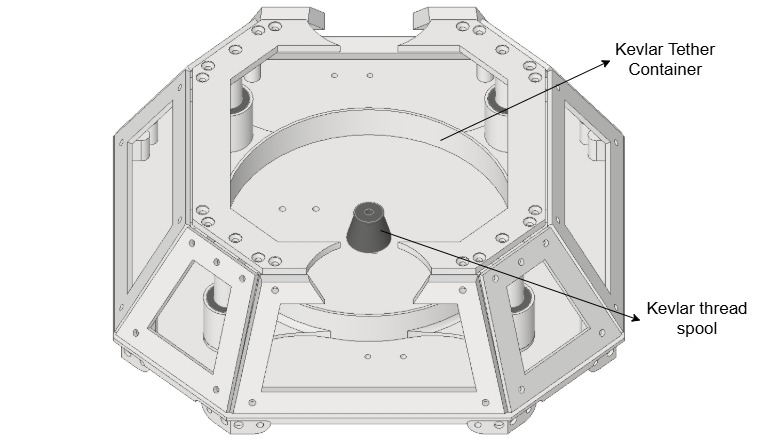
\includegraphics[width=1\linewidth]{PUCP_pictures/Assembly of the container and spool within the SATB structure.jpg}
    \caption{Assembly of the tether container and spool within the SAT-B structure.}
    \label{fig:container_spool_satb_assembly}
\end{figure}

The available volume for tether storage is estimated by subtracting the volume occupied by the spool from the cylindrical container volume:

\begin{equation}
V_{\mathrm{avail}}
=
V_{\mathrm{container}} - V_{\mathrm{spool}} .
\label{eq:available_tether_storage_volume}
\end{equation}

For the selected cylindrical container, with radius \(r_c=5.1~\mathrm{cm}\) and height \(h_c=1.25~\mathrm{cm}\), the container volume is

\begin{equation}
V_{\mathrm{container}}
=
\pi r_c^2 h_c
=
\pi(5.1)^2(1.25)
\approx
102.1~\mathrm{cm^3}.
\label{eq:container_volume_value}
\end{equation}

The spool is approximated as a conical frustum with larger radius \(R_s=0.8~\mathrm{cm}\), smaller radius \(r_s=0.6~\mathrm{cm}\), and height \(h_s=1.25~\mathrm{cm}\). Its volume is

\begin{equation}
V_{\mathrm{spool}}
=
\frac{1}{3}\pi h_s
\left(
R_s^2 + R_s r_s + r_s^2
\right)
\approx
1.94~\mathrm{cm^3}.
\label{eq:spool_volume_value}
\end{equation}

Therefore,

\begin{equation}
V_{\mathrm{avail}}
\approx
102.1 - 1.94
\approx
100.2~\mathrm{cm^3}.
\label{eq:available_volume_value}
\end{equation}

The resulting available volume satisfies the preliminary storage requirement of approximately \(100~\mathrm{cm^3}\). Therefore, the current container and spool configuration provides sufficient volume for the nominal \(100~\mathrm{m}\) tether, while remaining compatible with the preliminary SAT-B internal accommodation constraints.

\section{Experiment Instrumentation}
\label{sec:experiment_instrumentation}

The tether experiment requires instrumentation to measure and observe the deployment process and the subsequent dynamics of the tethered system. The instrumentation considered at this stage includes tether tension sensors, relative positioning and the Stereo Vision System.

These instruments support the reconstruction of the deployment sequence, the comparison with numerical simulations and ground tests, and the validation of key dynamic events such as tether release, tension build-up, possible rebound, and slack--tension transitions.

\subsection{Tether Tension Measurement}
\label{sub:tether_tension_measurement}

Tether tension is one of the main quantities required to characterize the mechanical behavior of the SAT-B/SAT-C tethered system. The current instrumentation concept considers force sensors at both tether ends, integrated into SAT-B and SAT-C, to measure slack-to-taut transitions, loads near full extension, and the subsequent dynamic response of the tethered configuration. This subsection presents the preliminary sensor selection and the proposed mechanical routing required to transmit the tether tension to the sensors.

\subsubsection{Tension Sensor Selection}
\label{subsub:tension_sensor_selection}

The tension sensor must be selected according to the expected load range, required resolution, environmental constraints, and available integration volume. At this stage, the preliminary selection criteria are:

\begin{itemize}
    \item Expected measurement range: \(0\)--\(2~\mathrm{N}\).
    \item Resolution: \(0.01~\mathrm{N}\) desirable.
    \item Mechanical overload capability: up to \(30~\mathrm{N}\) desirable, considering possible transient loads.
    \item Operating temperature range: \(-65~^\circ\mathrm{C}\) to \(120~^\circ\mathrm{C}\) desirable for flight compatibility.
\end{itemize}

Several sensing technologies were considered for tether tension measurement, including piezoelectric, optical, capacitive, and piezoresistive sensors. For the current concept, piezoresistive load cells were identified as the most suitable option because they provide direct force measurement, simple signal conditioning, compact form factors, and compatibility with laboratory tests. Optical and capacitive alternatives were not prioritized at this stage due to their higher integration and calibration complexity.

Several commercial load-cell options were reviewed for preliminary testing and integration assessment. Table~\ref{tab:tension_sensor_candidates} summarizes representative models identified during this search.

\begin{table}[htbp]
\centering
\caption{Representative load-cell candidates for tether tension measurement.}
\label{tab:tension_sensor_candidates}
\small
\renewcommand{\arraystretch}{1.2}
\begin{tabular}{|c|c|c|c|}
\hline
Provider & Device Code & Maximum Supported Force & Temperature Range \\ \hline
Interface Force & ULC-2N & \(10~\mathrm{N}\) & \(-15\) to \(50~^\circ\mathrm{C}\) \\ \hline
Futek & LSB205-S & \(2.5~\mathrm{N}\) & \(-50\) to \(93~^\circ\mathrm{C}\) \\ \hline
Ritcl & T303 & \(50~\mathrm{N}\) & \(-10\) to \(70~^\circ\mathrm{C}\) \\ \hline
HBK & U9C & \(50~\mathrm{N}\) & \(-10\) to \(70~^\circ\mathrm{C}\) \\ \hline
Althen & FN3280 & \(1.2\) or \(5~\mathrm{N}\) & \(-20\) to \(80~^\circ\mathrm{C}\) \\ \hline
LoadCellCentral & JRS1 & \(>2.5~\mathrm{N}\) & \(-10\) to \(40~^\circ\mathrm{C}\) \\ \hline
\end{tabular}
\end{table}

Among the evaluated options, the Futek LSB205-S and the Interface Force ULC-2N are relevant candidates for the current development stage. The Futek LSB205-S is considered as the current reference sensor for laboratory tests and preliminary mechanical integration because of its compact size and measurement range close to the expected tether tension range. However, the final sensor selection must still consider overload capability, calibration, thermal behavior, mechanical accommodation, and compatibility with the flight electronics. Figure~\ref{fig:futek_lsb205_sensor} shows the reference force sensor.

\begin{figure}[htbp]
    \centering
    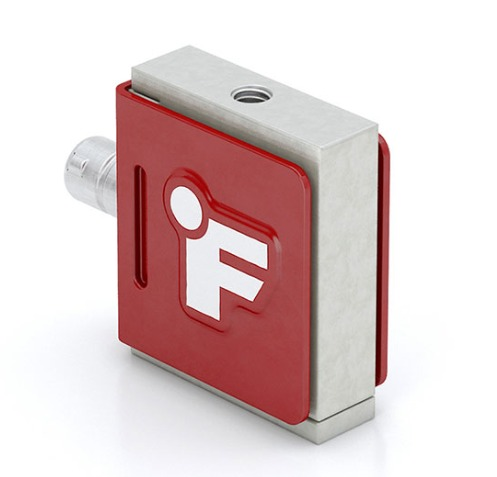
\includegraphics[width=0.3\linewidth]{PUCP_pictures/Fluke LSB205-S force sensor.jpeg}
    \caption{Futek LSB205-S force sensor considered as reference for preliminary tether tension measurement.}
    \label{fig:futek_lsb205_sensor}
\end{figure}

\subsubsection{Force Sensor Assembly in SAT-B and SAT-C}
\label{subsub:force_sensor_assembly}

Two force sensors are considered to measure tether tension at both ends. Their integration into SAT-B and SAT-C must minimize occupied volume and remain compatible with other subsystems, including the EPS, OBC, communication equipment, and the tether storage and deployment mechanism.

In SAT-B, a horizontal sensor orientation was initially considered to reduce the occupied height. However, the reference load cell measures force along its primary loading axis, as shown in Figure~\ref{fig:lsb205_measurement_direction}. Therefore, a force transmission path is required to redirect the tether tension toward the sensor loading axis.

\begin{figure}[htbp]
    \centering
    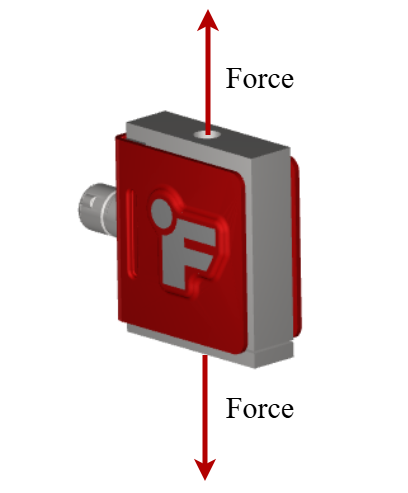
\includegraphics[width=0.3\linewidth]{PUCP_pictures/Example of the measurement direction of the SB205-S force sensor.png}
    \caption{Reference loading direction of the LSB205-S force sensor.}
    \label{fig:lsb205_measurement_direction}
\end{figure}

To address this integration constraint, the tether is routed through a pulley before reaching the force sensor. This routing redirects the force direction, allowing the sensor to be mounted horizontally while the tether exits SAT-B along the deployment direction. The pulley introduces friction losses and possible measurement bias; therefore, calibration tests will be required to quantify these effects and define an appropriate correction factor. The proposed sensor and pulley location within SAT-B is shown in Figure~\ref{fig:satb_force_sensor_pulley_location}.

\begin{figure}[htbp]
    \centering
    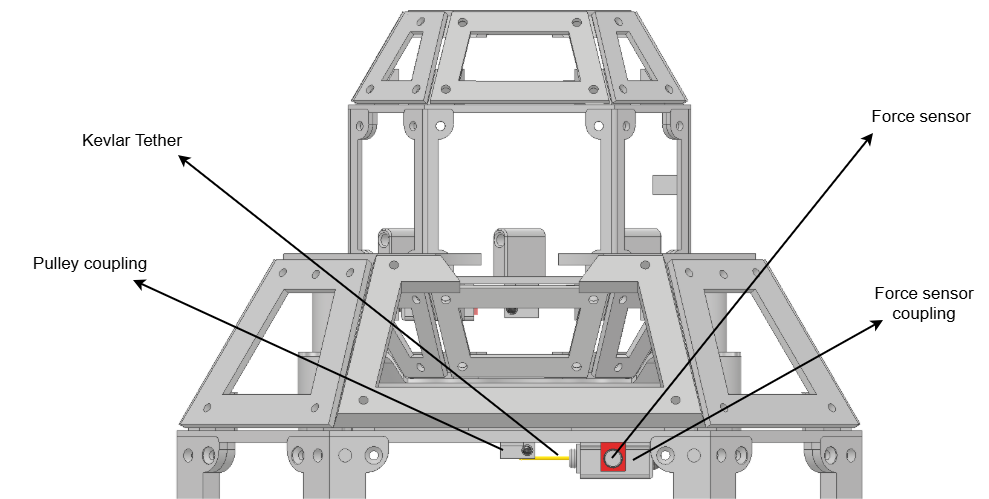
\includegraphics[width=1\linewidth]{PUCP_pictures/Location of the force sensor and pulley within the SATB structure.png}
    \caption{Location of the force sensor and pulley within the SAT-B structure.}
    \label{fig:satb_force_sensor_pulley_location}
\end{figure}

Both the force sensor and the pulley include dedicated mounts for integration into the SAT-B structure, using the octagonal base of SAT-B as the mechanical reference. Figure~\ref{fig:satb_force_sensor_pulley_front_view} shows a front view of the proposed sensor and pulley assembly.

\begin{figure}[htbp]
    \centering
    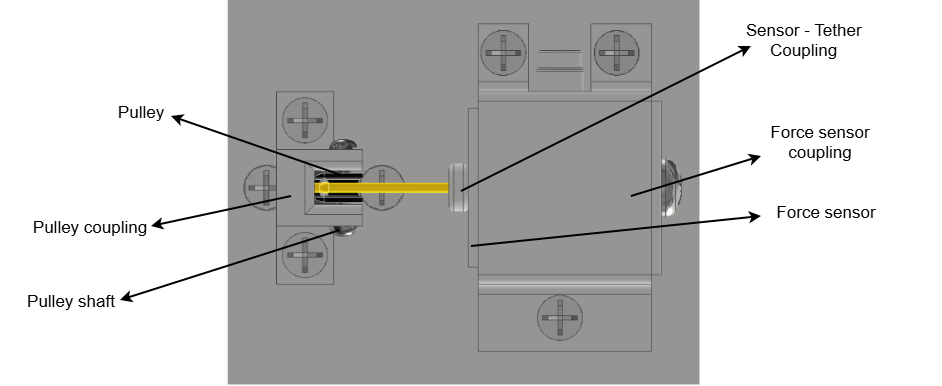
\includegraphics[width=1\linewidth]{PUCP_pictures/Front view of the force sensor and pulley assembly within the SATB structure.png}
    \caption{Front view of the force sensor and pulley assembly within the SAT-B structure.}
    \label{fig:satb_force_sensor_pulley_front_view}
\end{figure}

The assembly requires a coupling element between the force sensor and the tether end. After passing through the pulley, the tether is routed through a hole located near the center of the SAT-B octagonal base, allowing it to continue toward the storage container and deployment path.

The SAT-C implementation follows the same measurement principle. A second force sensor and pulley redirect the tether force toward the sensor loading axis while maintaining the tether path along the common separation direction between SAT-B and SAT-C. Figure~\ref{fig:satbc_tether_routing} shows the complete tether routing between SAT-B and SAT-C, including the pulleys, storage container, and sensor connection points.

\begin{figure}[htbp]
    \centering
    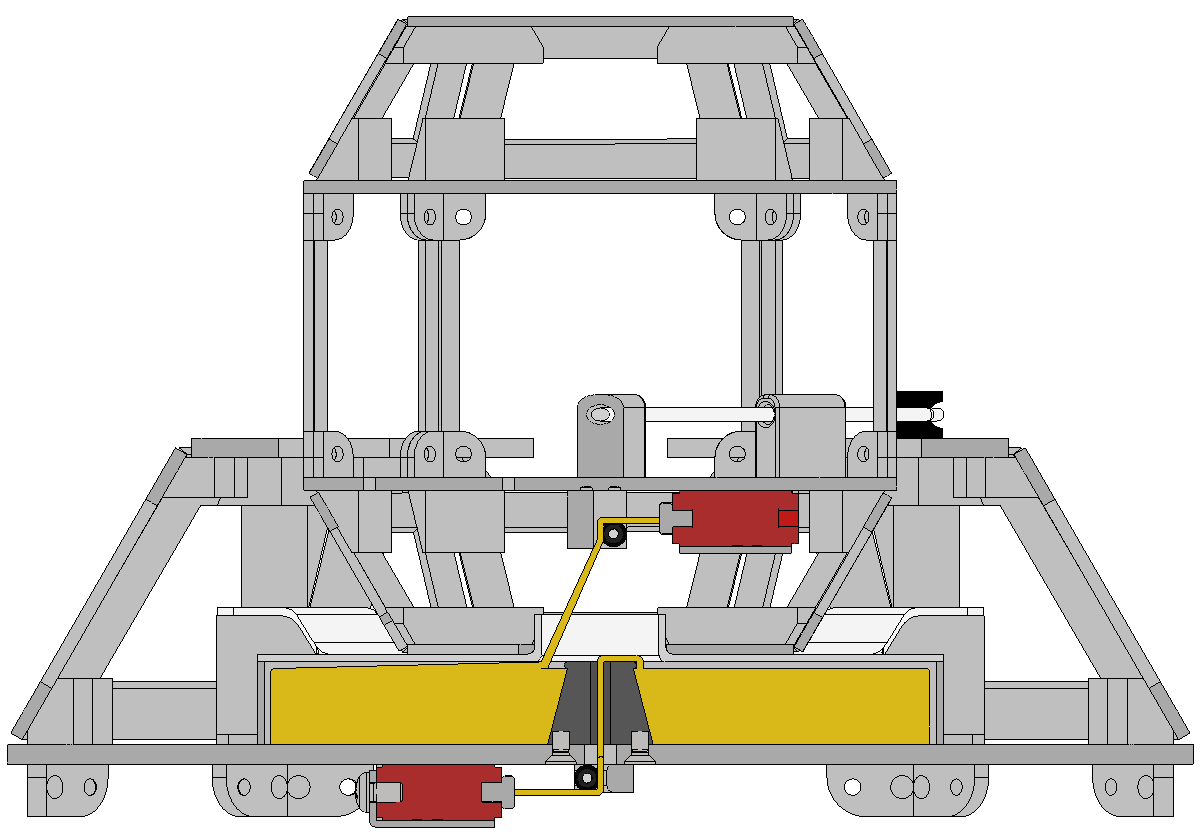
\includegraphics[width=0.8\linewidth]{PUCP_pictures/corte_recorrido_hilo_kevlar.png}
    \caption{Cross-sectional view of the tether routing and force sensor integration between SAT-B and SAT-C.}
    \label{fig:satbc_tether_routing}
\end{figure}

\subsection{Relative Positioning}
\label{sub:relative_positioning_time_sync}

Relative positioning for the tether experiment is supported by GNSS receivers installed on both SAT-B and SAT-C. The time-tagged position data from each satellite provide the basis for estimating the SAT-B/SAT-C relative-position vector during and after tether deployment:

\begin{equation}
    \mathbf{r}_{BC}(t) = \mathbf{r}_{C}(t) - \mathbf{r}_{B}(t),
\end{equation}

where \(\mathbf{r}_{B}(t)\) and \(\mathbf{r}_{C}(t)\) are the GNSS-derived position vectors of SAT-B and SAT-C, respectively. This information supports the analysis of the tethered-system motion and provides a common time reference for correlating GNSS data with camera images, tether-tension measurements, and housekeeping telemetry.

The GNSS measurements do not directly determine the tether geometry. Instead, they provide the relative-state history of the two satellites, while the tether shape and deployment condition are assessed mainly from camera observations and tension measurements. The combined dataset is intended for ground-based post-processing and comparison with the pre-flight tether-dynamics simulations. The GNSS sampling interval should be configurable according to the mission stage. A higher sampling rate should be used during SAT-B/SAT-C separation and tether deployment, when the relative motion changes more rapidly. During stable tethered-system observation, the sampling rate can be reduced to limit data volume and power consumption.

The GNSS receivers and antennas must be compatible with LEO operation and with the SAT-B and SAT-C accommodation constraints. The next design stage should consolidate the receiver selection, antenna placement, expected positioning accuracy, data format, synchronization approach, and integration with the camera and tension-sensor data streams.

                    
\newpage
\subsection{Stereo Vision System Concept}
\label{sub:stereo_vision_concept}

The Stereo Vision System is part of the instrumentation of the LINKU tether experiment. It is intended to observe the evolution of the system from the initial SAT-BC configuration to the nominal maximum separation between SAT-B and SAT-C, as illustrated in Figure~\ref{fig:overview-stereo-camera}. The main events of interest are the SAT-B/SAT-C separation, the progressive release of the tether, and the spatial configuration of the tethered system, including the visible path of the tether between both satellites. This supports the use of image-based reconstruction techniques to estimate the tether geometry in orbit.

The Stereo Vision System complements the other measurements considered for the tether experiment. Tether-tension sensors provide local force information at the attachment points, while relative positioning measurements provide satellite-level separation information. However, these measurements do not directly describe the spatial geometry of the tether between SAT-B and SAT-C. The Stereo Vision System is therefore included to provide image-based information for deployment monitoring, tether geometry reconstruction, and the interpretation of possible deployment events.

\begin{figure}[htbp]
    \centering
    \begin{subfigure}{0.49\textwidth}
        \centering
        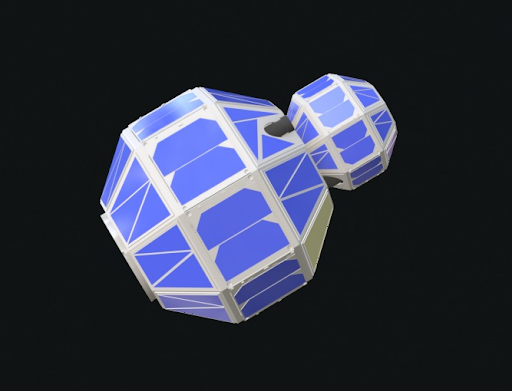
\includegraphics[
            height=5.75cm,
            keepaspectratio
        ]{PUCP_pictures/Stereo vision system/Figure1.1a.png}
        \caption{}
        \label{fig:first_stage}
    \end{subfigure}
    \hfill
    \begin{subfigure}{0.49\textwidth}
        \centering
        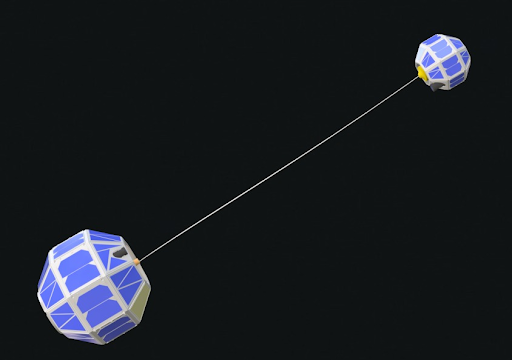
\includegraphics[
            height=5.75cm,
            keepaspectratio
        ]{PUCP_pictures/Stereo vision system/Figure1.1b.png}
        \caption{}
        \label{fig:second_stage}
    \end{subfigure}
    \caption{Reference configurations of the tethered system:
    (a) SAT-B and SAT-C before separation;
    (b) SAT-B and SAT-C at nominal maximum separation, not to scale.}
    \label{fig:overview-stereo-camera}
\end{figure}

The system is based on synchronized stereo image acquisition and geometry-driven reconstruction methods. As summarized in Figure~\ref{fig:figure1.2}, the Stereo Vision System acquires stereo image pairs, processes the observed tether geometry, and supports the reconstruction of three-dimensional information from visual data. This approach is necessary because the tether is expected to appear as a thin, low-texture structure against a dark orbital background, making conventional texture-based photogrammetry insufficient. Instead, the proposed approach combines geometric continuity, radiometric contrast, centerline extraction, stereo correspondence, and constrained triangulation.

\begin{landscape}
\begin{figure}[htbp]
    \centering
    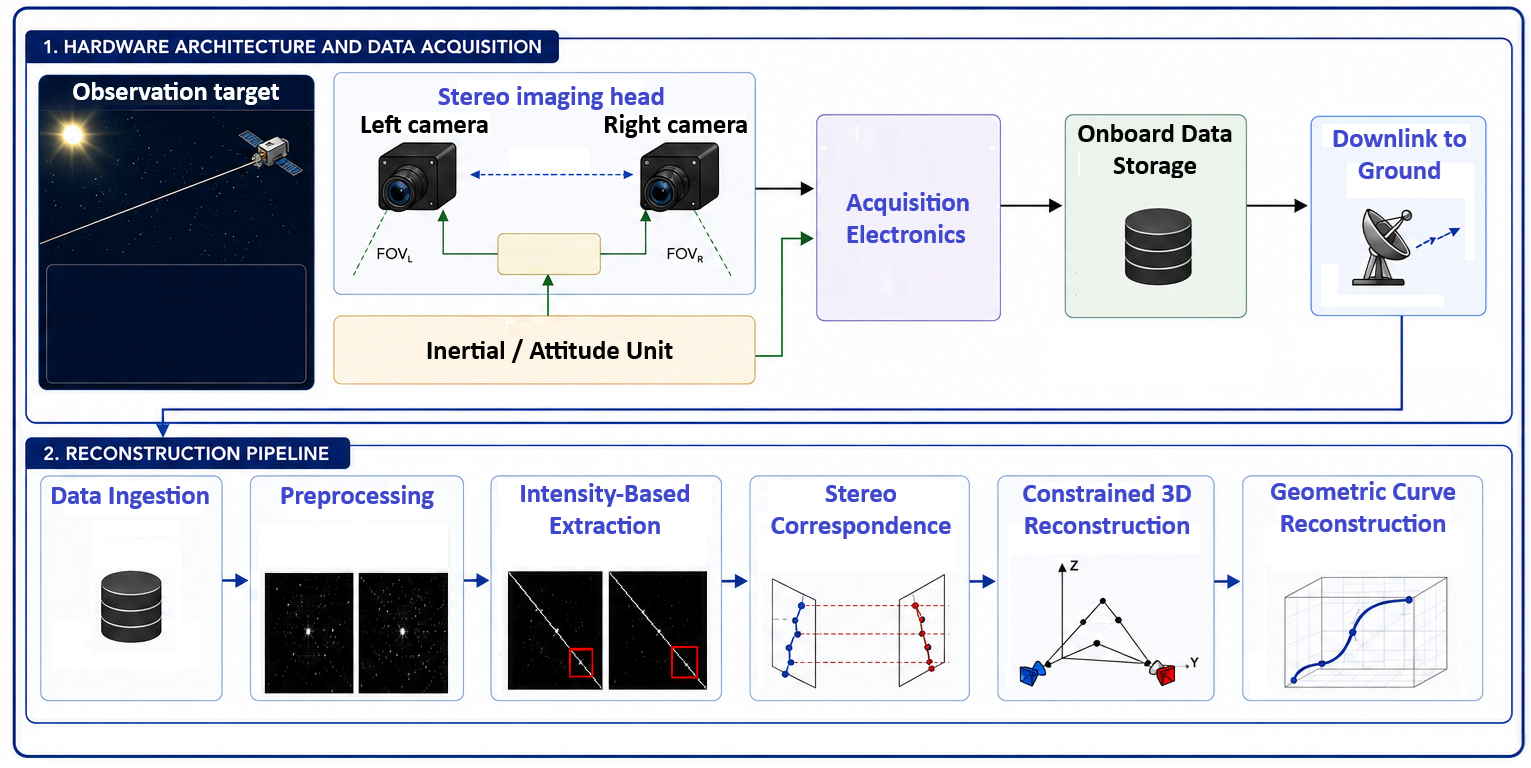
\includegraphics[width=\linewidth]{PUCP_pictures/Stereo vision system/Figure1.2.png}
    \caption[Stereo Vision System architecture and reconstruction pipeline.]{Stereo Vision System architecture and reconstruction pipeline. The diagram summarizes stereo image acquisition, geometry-driven reconstruction, and the main outputs used for tether reconstruction.}
    \label{fig:figure1.2}
\end{figure}
\end{landscape}

\subsubsection{Stereo Vision Cameras and Accommodation}
\label{subsub:stereo_vision_camera_accommodation}

This subsection describes the reference camera model, the preliminary camera locations, and the main mechanical constraints associated with the integration of the cameras and sunshades in SAT-B and SAT-C.

For the current accommodation prototype, the \(12~\mathrm{MP}\) Arducam module based on the IMX708 sensor is used as the reference camera. This selection is consistent with the preliminary optical and reconstruction analyses described later in this section, while its compact size facilitates integration within the limited available volume of SAT-B and SAT-C.

In SAT-B, the cameras are located along the longest edges of the upper section of the structure. Since these edges are inclined, the mounting design must adapt to the dodecahedral geometry while preserving a smooth external envelope. This reduces external protrusions and helps lower the risk of tether contact or entanglement during deployment. The cameras are positioned between the outer diameter of the tether container and the largest upper face of SAT-B, as shown in Figure~\ref{fig:satb_arducam_location}.

\begin{figure}[htbp]
    \centering
    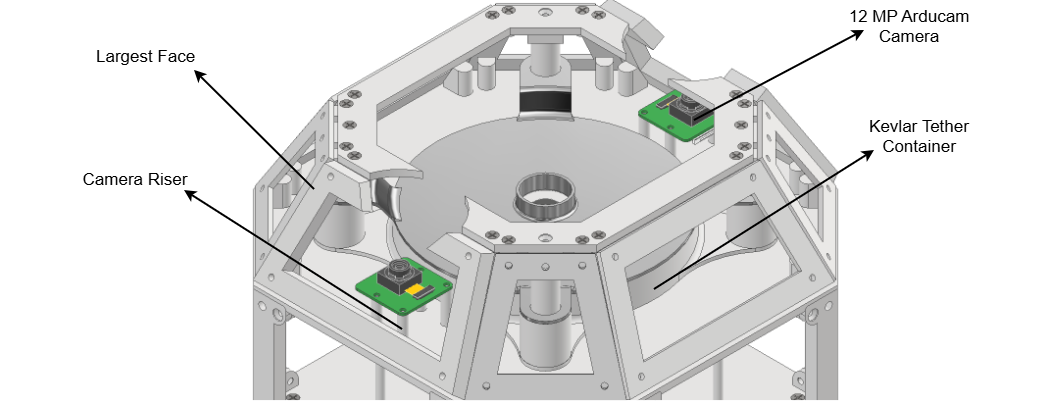
\includegraphics[width=0.95\linewidth]{PUCP_pictures/Location of the 12 MP Arducam camera on the upper part of SATB.png}
    \caption{Location of the \(12~\mathrm{MP}\) Arducam camera on the upper section of SAT-B.}
    \label{fig:satb_arducam_location}
\end{figure}

The cameras are mounted on the upper octagonal base of SAT-B using spacers. These spacers increase the camera height and reduce obstruction by nearby structural elements. The largest upper face of SAT-B is locally thickened to accommodate the camera assembly within the available volume.

Cutouts are included in the adjacent face and in the top cover of SAT-B to preserve the camera field of view and support the integration of a sunshade. The sunshade is intended to reduce direct solar illumination on the camera lens. Its geometry was defined considering the approximate \(80^\circ\) field of view of the reference camera and the available height in the upper section of SAT-B. The resulting camera and sunshade assembly is shown in Figure~\ref{fig:satb_camera_sunshade_assembly}.

\begin{figure}[htbp]
    \centering
    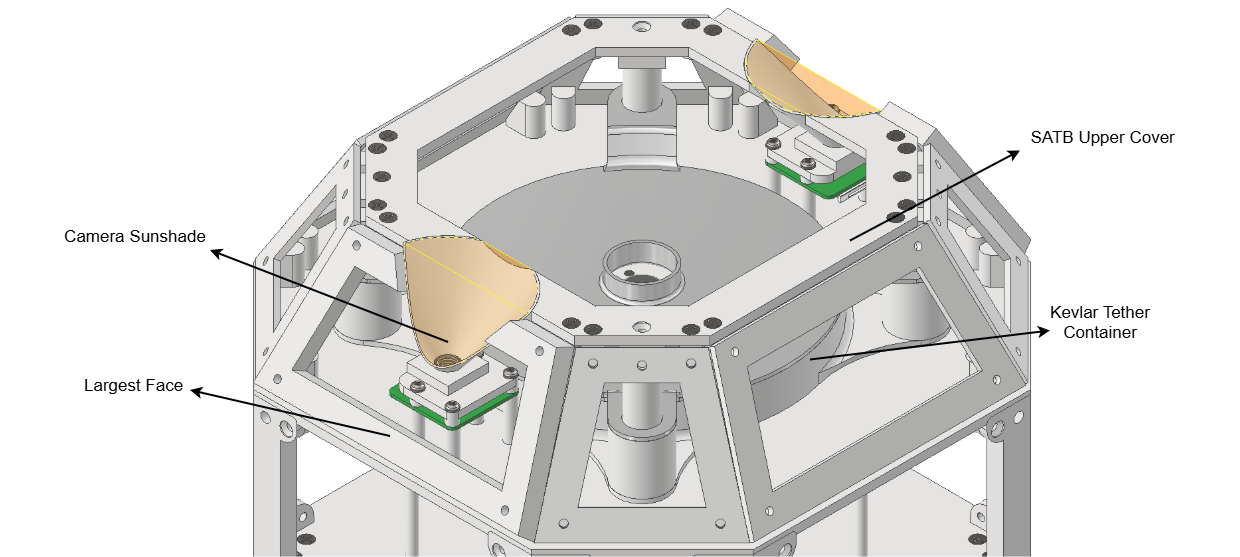
\includegraphics[width=0.95\linewidth]{PUCP_pictures/Assembly of the cameras with the sunshade.png}
    \caption{Camera and sunshade assembly in SAT-B.}
    \label{fig:satb_camera_sunshade_assembly}
\end{figure}

The sunshade is attached to the cutout regions near the camera and to the top cover of SAT-B. This provides additional mechanical support compared with a mounting based only on the camera board screws and standoffs. A cross-sectional view of the assembly is shown in Figure~\ref{fig:satb_camera_sunshade_section}.

\begin{figure}[htbp]
    \centering
    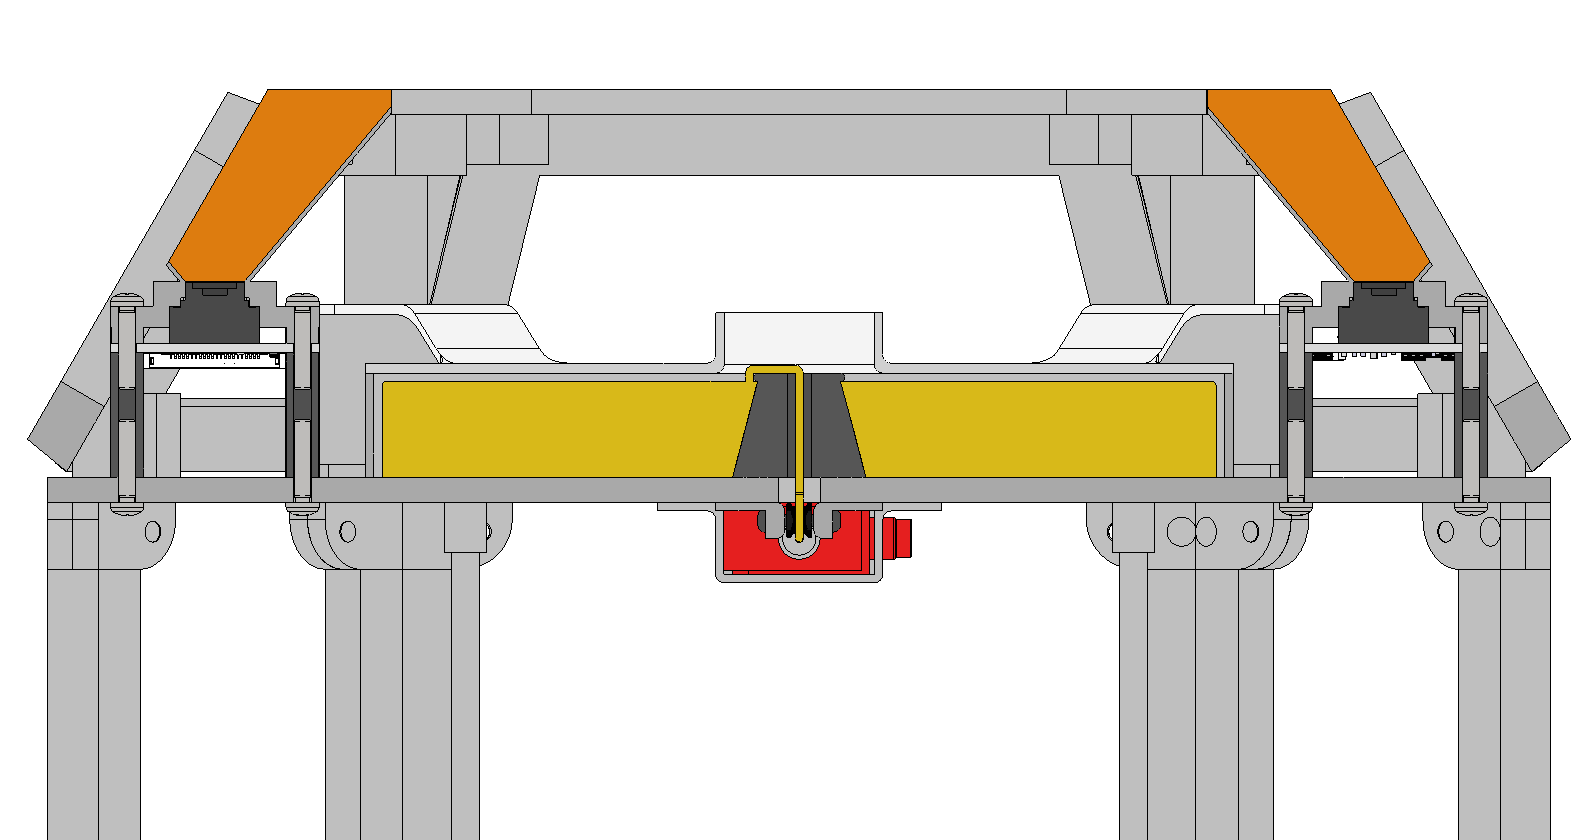
\includegraphics[width=0.8\linewidth]{PUCP_pictures/Cross-sectional view of the camera assembly with the sunshade.png}
    \caption{Cross-sectional view of the camera and sunshade assembly in SAT-B.}
    \label{fig:satb_camera_sunshade_section}
\end{figure}

The cross-sectional view confirms that the camera, screws, spacers, and sunshade remain within the SAT-B geometric envelope. Therefore, the proposed assembly remains compatible with the external panels and the tether deployment environment.

In SAT-C, the available space allows the installation of one camera in the upper section of the satellite. The assembly follows the same principle used for SAT-B: the camera is mounted using spacers, and the sunshade is adapted to the dodecahedral geometry. The proposed SAT-C camera and sunshade assembly is shown in Figure~\ref{fig:satc_camera_sunshade_assembly}.

\begin{figure}[htbp]
    \centering
    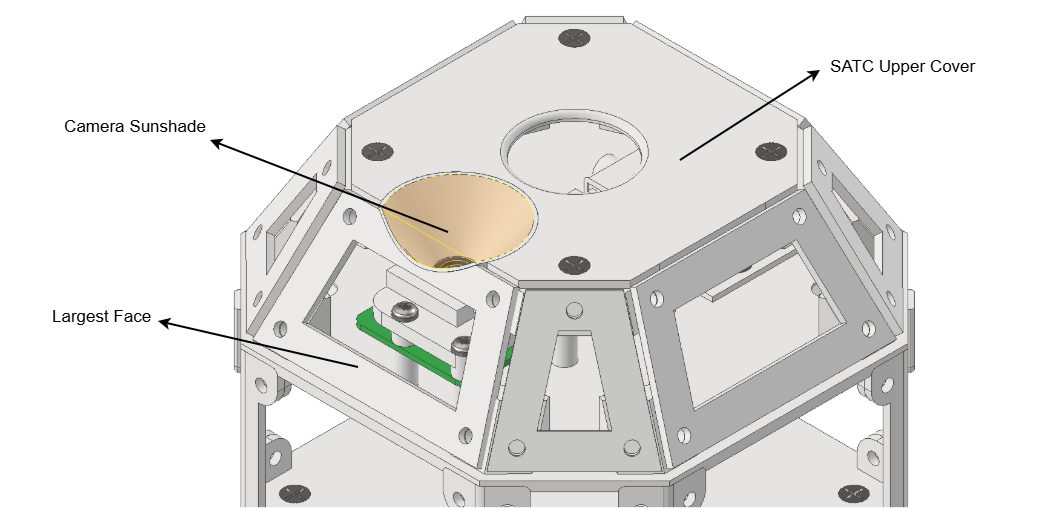
\includegraphics[width=1\linewidth]{PUCP_pictures/Assembly of the cameras with the sunshade in the SATC.png}
    \caption{Camera and sunshade assembly in SAT-C.}
    \label{fig:satc_camera_sunshade_assembly}
\end{figure}

The SAT-C assembly was also checked using a cross-sectional view to verify that the sunshade and mounting elements remain within the limits defined by the inclined faces of the structure. This verification is shown in Figure~\ref{fig:satc_camera_sunshade_section}.

\begin{figure}[htbp]
    \centering
    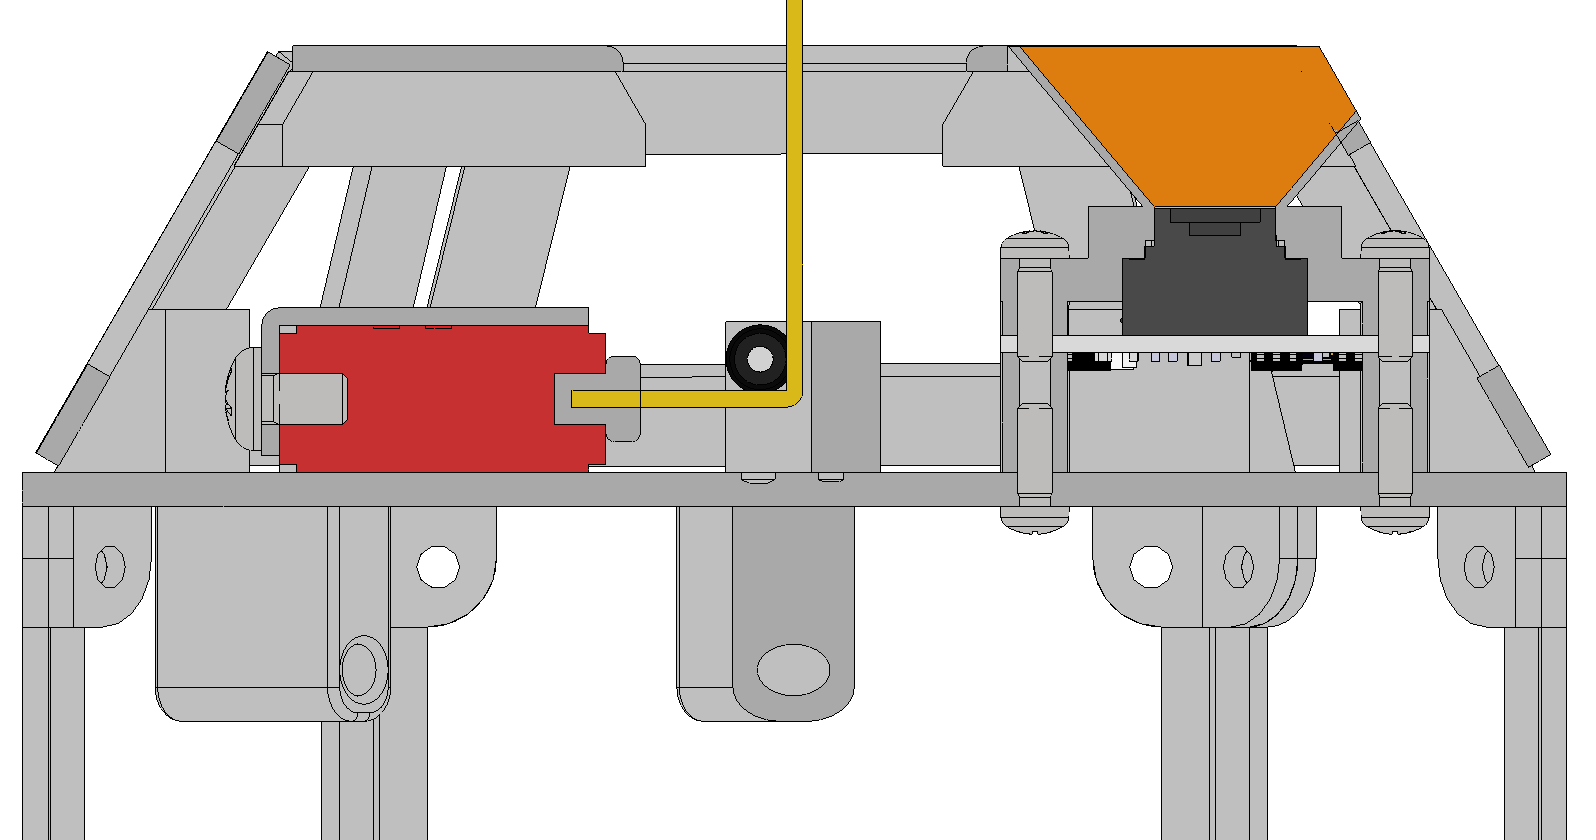
\includegraphics[width=0.8\linewidth]{PUCP_pictures/Cross-sectional view of the camera assembly with the sunshade in the SATC.png}
    \caption{Cross-sectional view of the camera and sunshade assembly in SAT-C.}
    \label{fig:satc_camera_sunshade_section}
\end{figure}

The cross-sectional view indicates that the camera and sunshade remain within the SAT-C geometric envelope. Unlike SAT-B, the SAT-C camera face does not require local thickening, since SAT-C does not include the tether container or the separation mechanism within the same internal region.

\newpage
\subsubsection{Objectives of the Stereo Vision System}
\label{subsub:stereo_vision_objectives}

The objectives of the Stereo Vision System are directly related to the operational needs of the LINKU tether experiment. Its primary mission-level objectives are:

\begin{itemize}
    \item To verify the nominal deployment of the tether and identify possible anomalies during the separation process between SAT-B and SAT-C.
    \item To characterize the three-dimensional spatial geometry of the tether during post-deployment operations.
    \item To support the interpretation of tether oscillations, curvature, and deployment events using image-based geometric information.
    \item To provide visual geometric information complementary to relative positioning and tether-tension measurements.
\end{itemize}

These objectives define the future operational role of the Stereo Vision System within the mission architecture. In this context, the system is conceived as a complementary observation instrument for deployment monitoring, anomaly detection, and post-deployment dynamic characterization.

\subsubsection{Scope of the Stereo Vision Analysis}
\label{subsub:stereo_vision_current_work_scope}

The objectives of the current work are different from the mission-level objectives of the Stereo Vision System. While the system is intended to support future LINKU mission operations, the present work evaluates the technical feasibility of the proposed stereo vision approach, identifies its main limitations, and provides a basis for the development and validation of future camera-system prototypes.

The scope of the current work follows a progressive validation strategy, summarized in Figure~\ref{fig:figure1.3}. This strategy begins with the analysis of a conventional photogrammetry baseline, continues with the validation of a geometry-driven reconstruction framework, and includes an exploratory assessment of AI-assisted reconstruction methods as future support tools.

The main objectives of the current work are:

\begin{itemize}
    \item To analyze the optical and radiometric constraints that affect tether observation under orbital-like conditions.
    \item To evaluate whether a thin tether-like structure can be detected and reconstructed under representative visual conditions.
    \item To compare conventional photogrammetry and geometry-driven stereo reconstruction.
    \item To assess the performance and limitations of exploratory AI-assisted reconstruction methods, establishing the boundaries of what AI-based techniques can reliably contribute to tether geometry recovery.
    \item To validate the feasibility of a geometry-driven reconstruction framework experimentally.
    \item To define the main technical steps required to continue the development and validation of future Stereo Vision System prototypes.
\end{itemize}

\begin{landscape}
\begin{figure}[htbp]
    \centering
    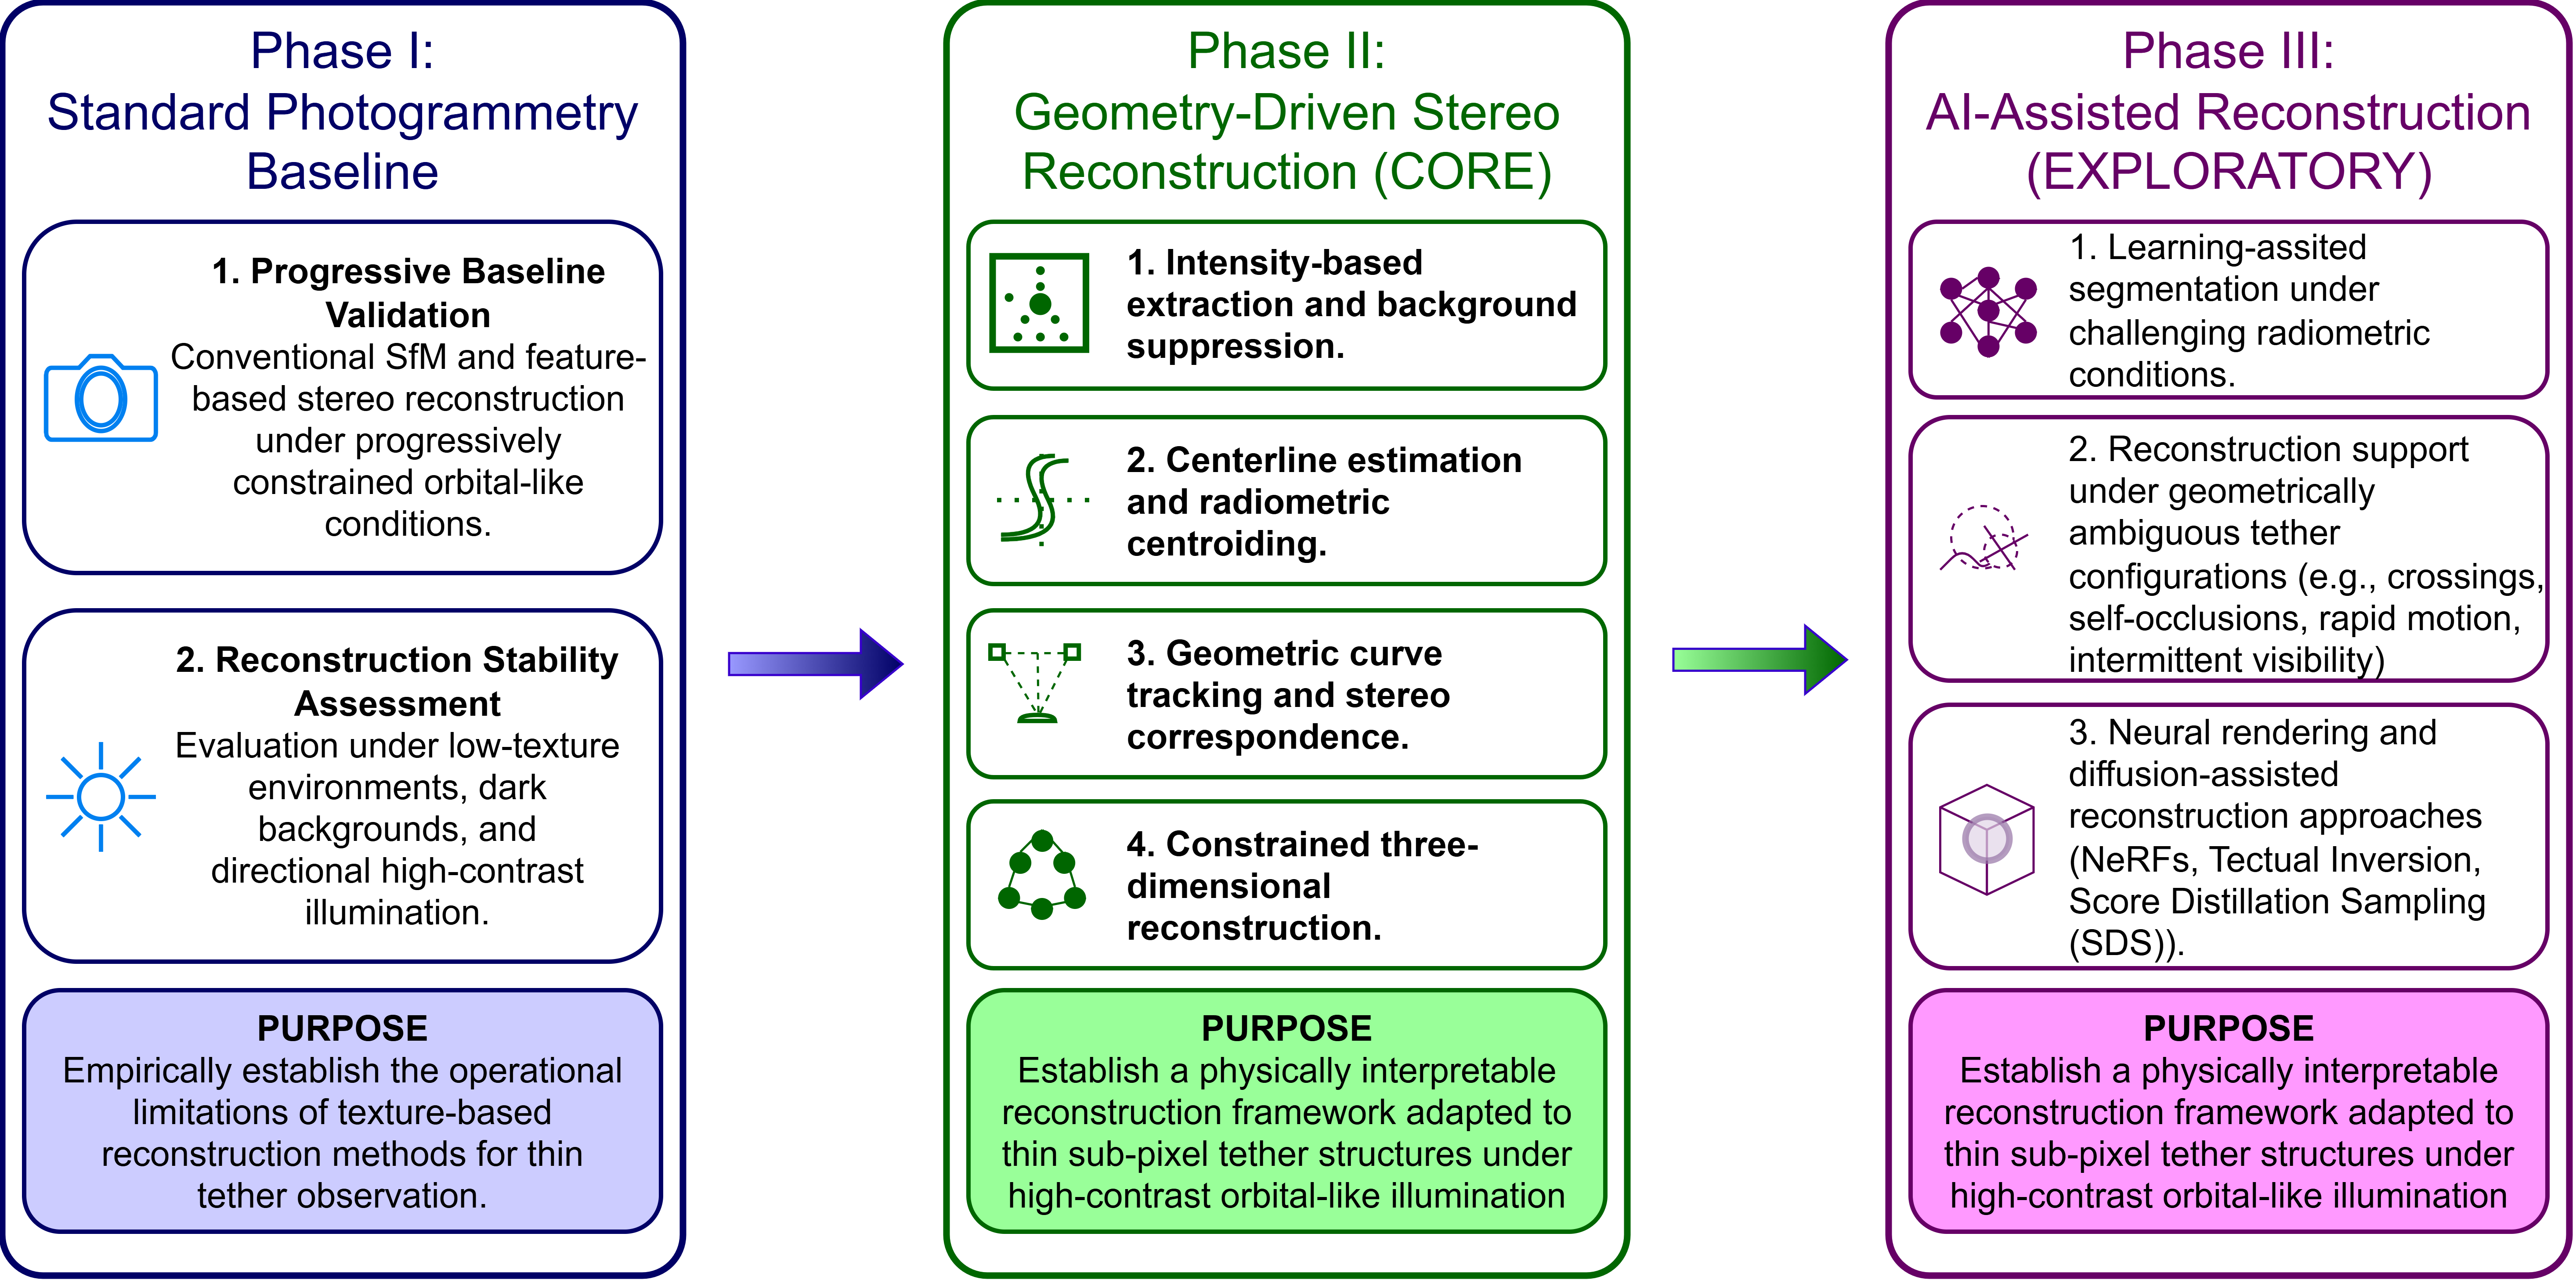
\includegraphics[width=0.95\linewidth]{PUCP_pictures/Stereo vision system/Figure1.3.png}
    \caption[Validation roadmap of the Stereo Vision System concept.]{Validation roadmap of the Stereo Vision System concept. The workflow progresses from conventional photogrammetry assessment to geometry-driven stereo reconstruction and exploratory AI-assisted support methods.}
    \label{fig:figure1.3}
\end{figure}
\end{landscape}

The central technical focus of the current work is the geometry-driven reconstruction approach. As illustrated in Figure~\ref{fig:figure1.4}, this methodology does not rely on conventional texture-based feature matching. Instead, it uses tether extraction, centerline estimation, stereo correspondence, and constrained three-dimensional reconstruction to recover the tether geometry from stereo images.

\begin{figure}[htbp]
    \centering
    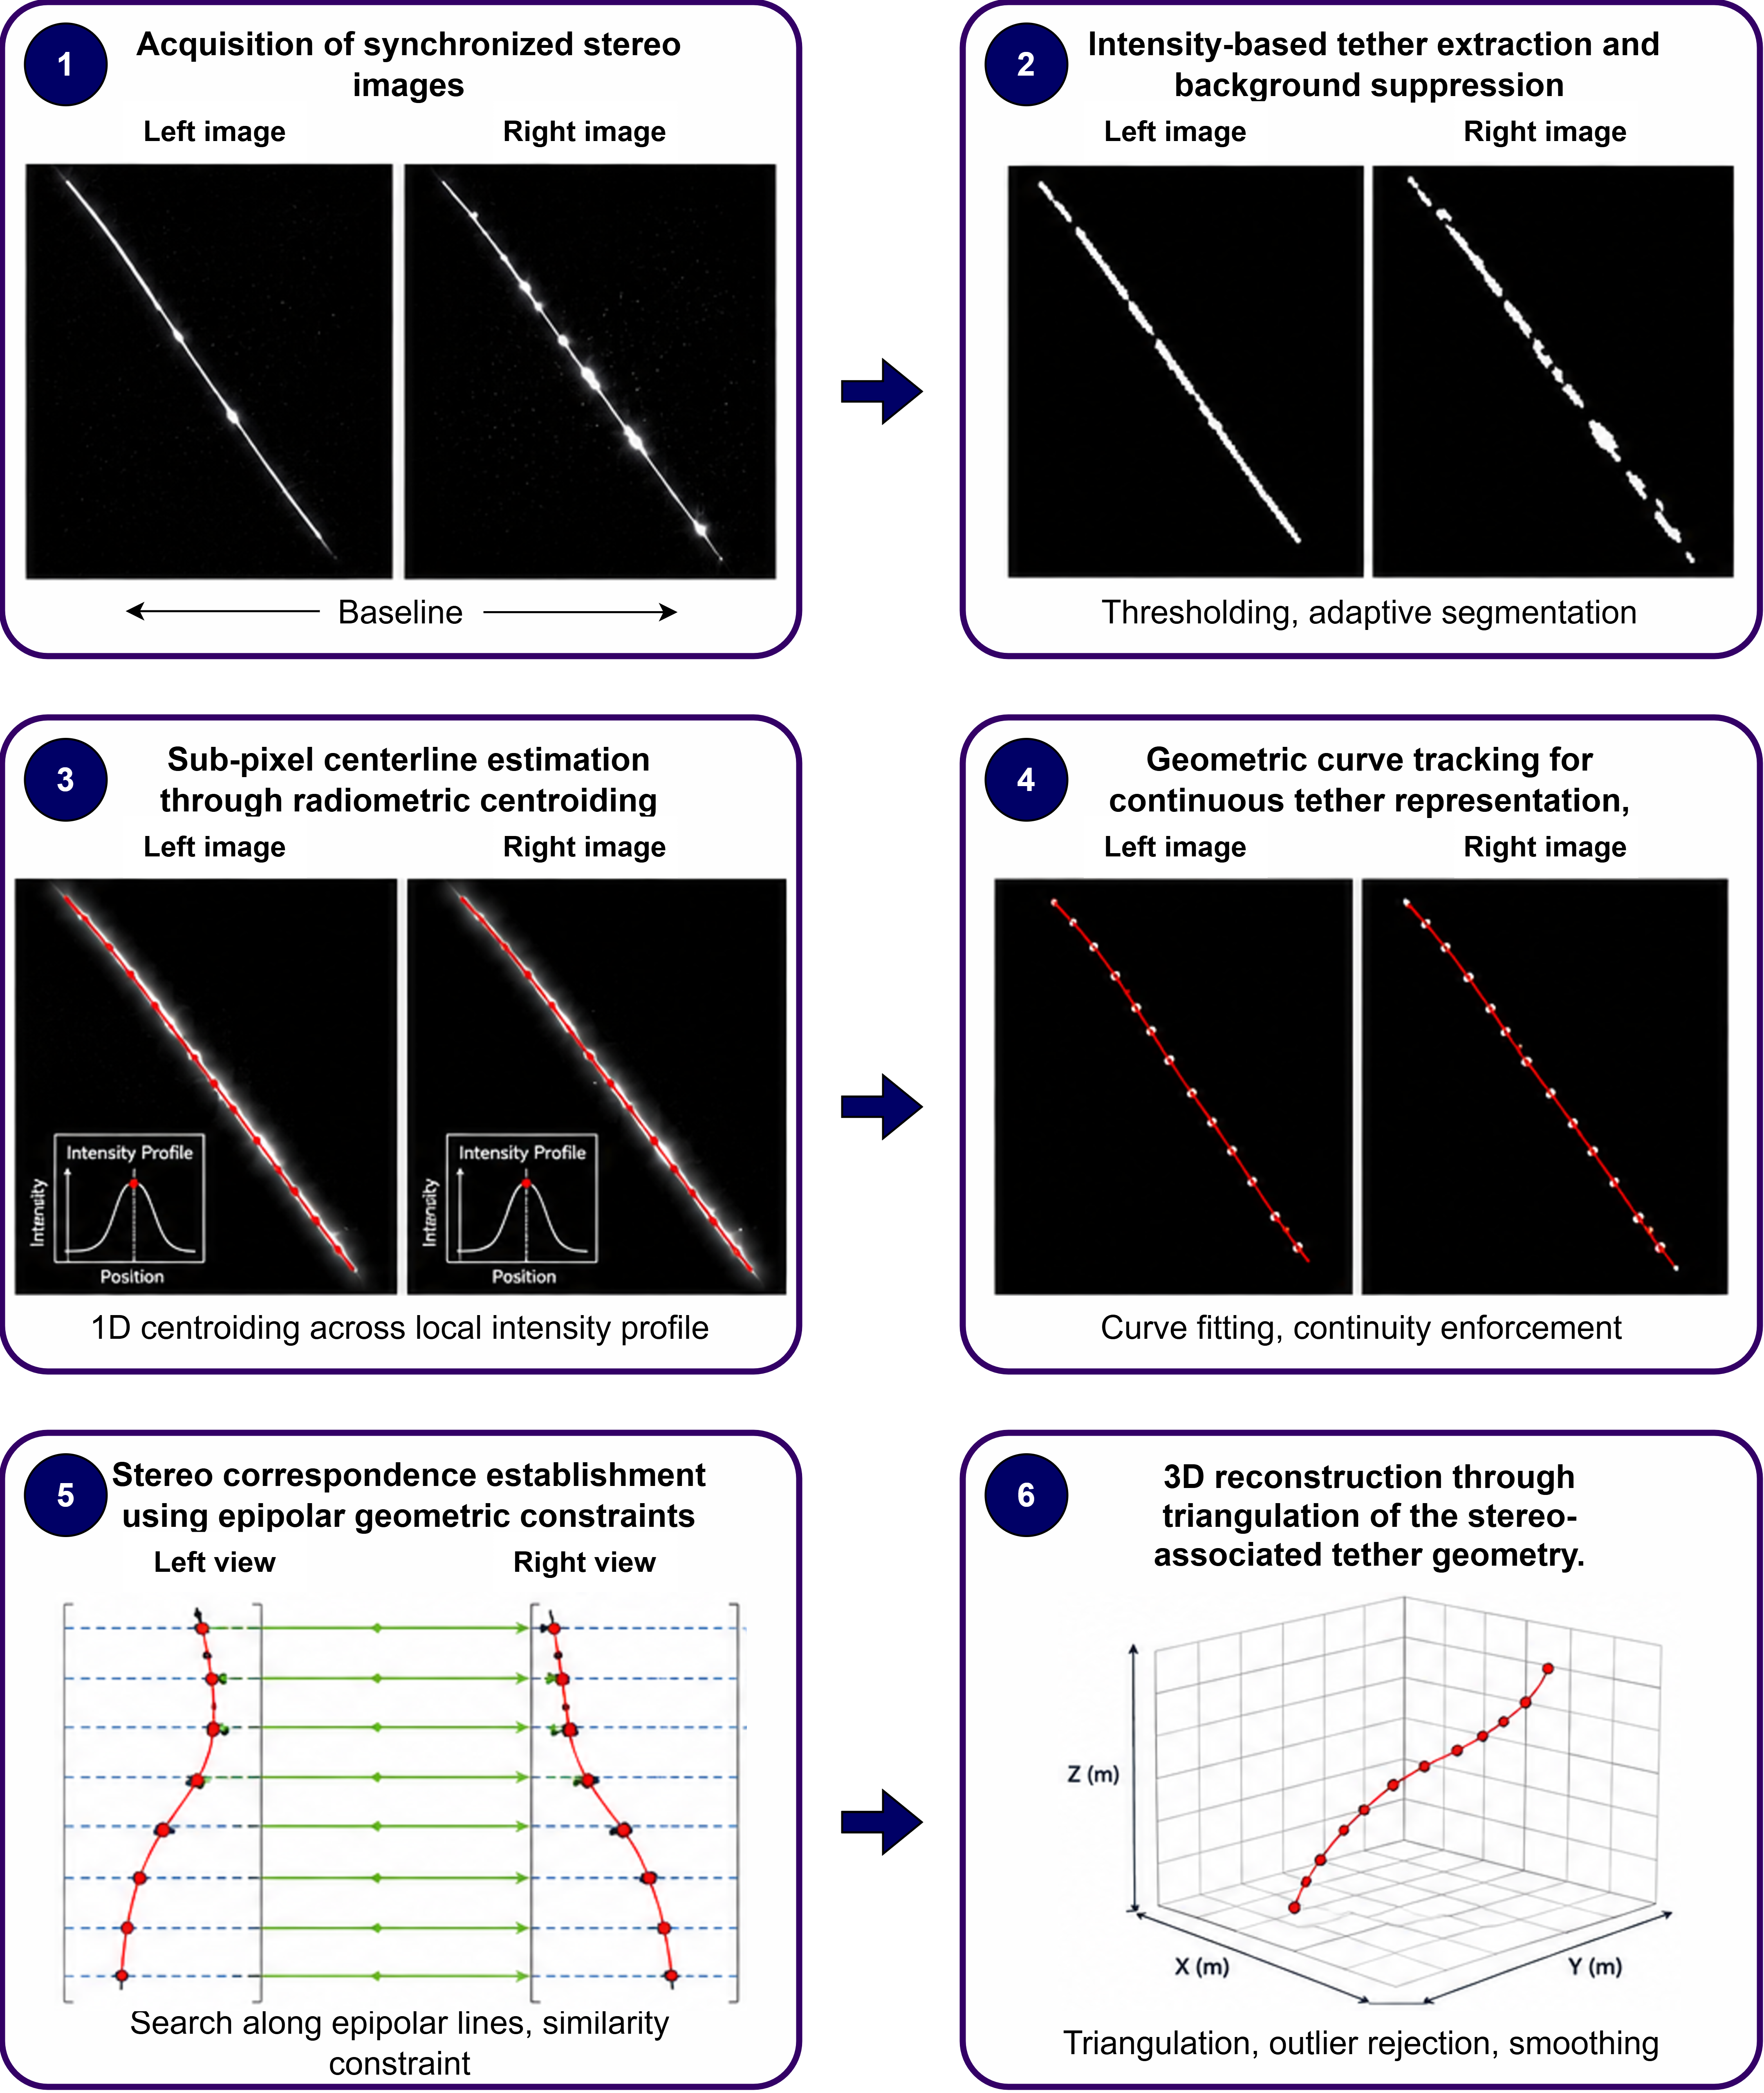
\includegraphics[width=\textwidth]{PUCP_pictures/Stereo vision system/Figure1.4.png}
    \caption{Geometry-driven tether reconstruction pipeline.}
    \label{fig:figure1.4}
\end{figure}

Therefore, the current work should be understood as a concept characterization and preliminary validation effort. It establishes the feasibility, limitations, and development path of the proposed LINKU Stereo Vision System architecture.

\newpage
\subsubsection{Tests and Analyses Performed}
\label{subsub:stereo_vision_tests_analyses}

The work followed a progressive validation strategy that combined theoretical analysis, laboratory testing, and comparative reconstruction assessment. The objective was to evaluate the feasibility of observing and reconstructing a thin tether-like structure under visual conditions representative of orbital operation.

\vspace{0.3cm}
\noindent\textbf{Optical and Theoretical Analysis}

The first stage involved analyzing the optical feasibility of tether observation. The study evaluated the relationship between field of view, pixel density, depth of field, geometric resolution, and long-range radiometric detectability. To support this analysis, a custom analytical tool was developed to compare representative COTS camera configurations and estimate the transition between the geometric detection regime and the sub-pixel radiometric regime.

The analysis showed that a millimeter-scale tether transitions from a geometrically resolvable object in the near field to a sub-pixel radiometric feature at long observation distances. At mission-relevant distances of approximately \(100~\mathrm{m}\), the tether cannot be treated as a fully resolved geometric object and must instead be detected through its radiometric response. This transition is conceptually summarized in Figures~\ref{fig:figure1.5a} and~\ref{fig:figure1.5b}.

\begin{figure}[htbp]
    \centering
    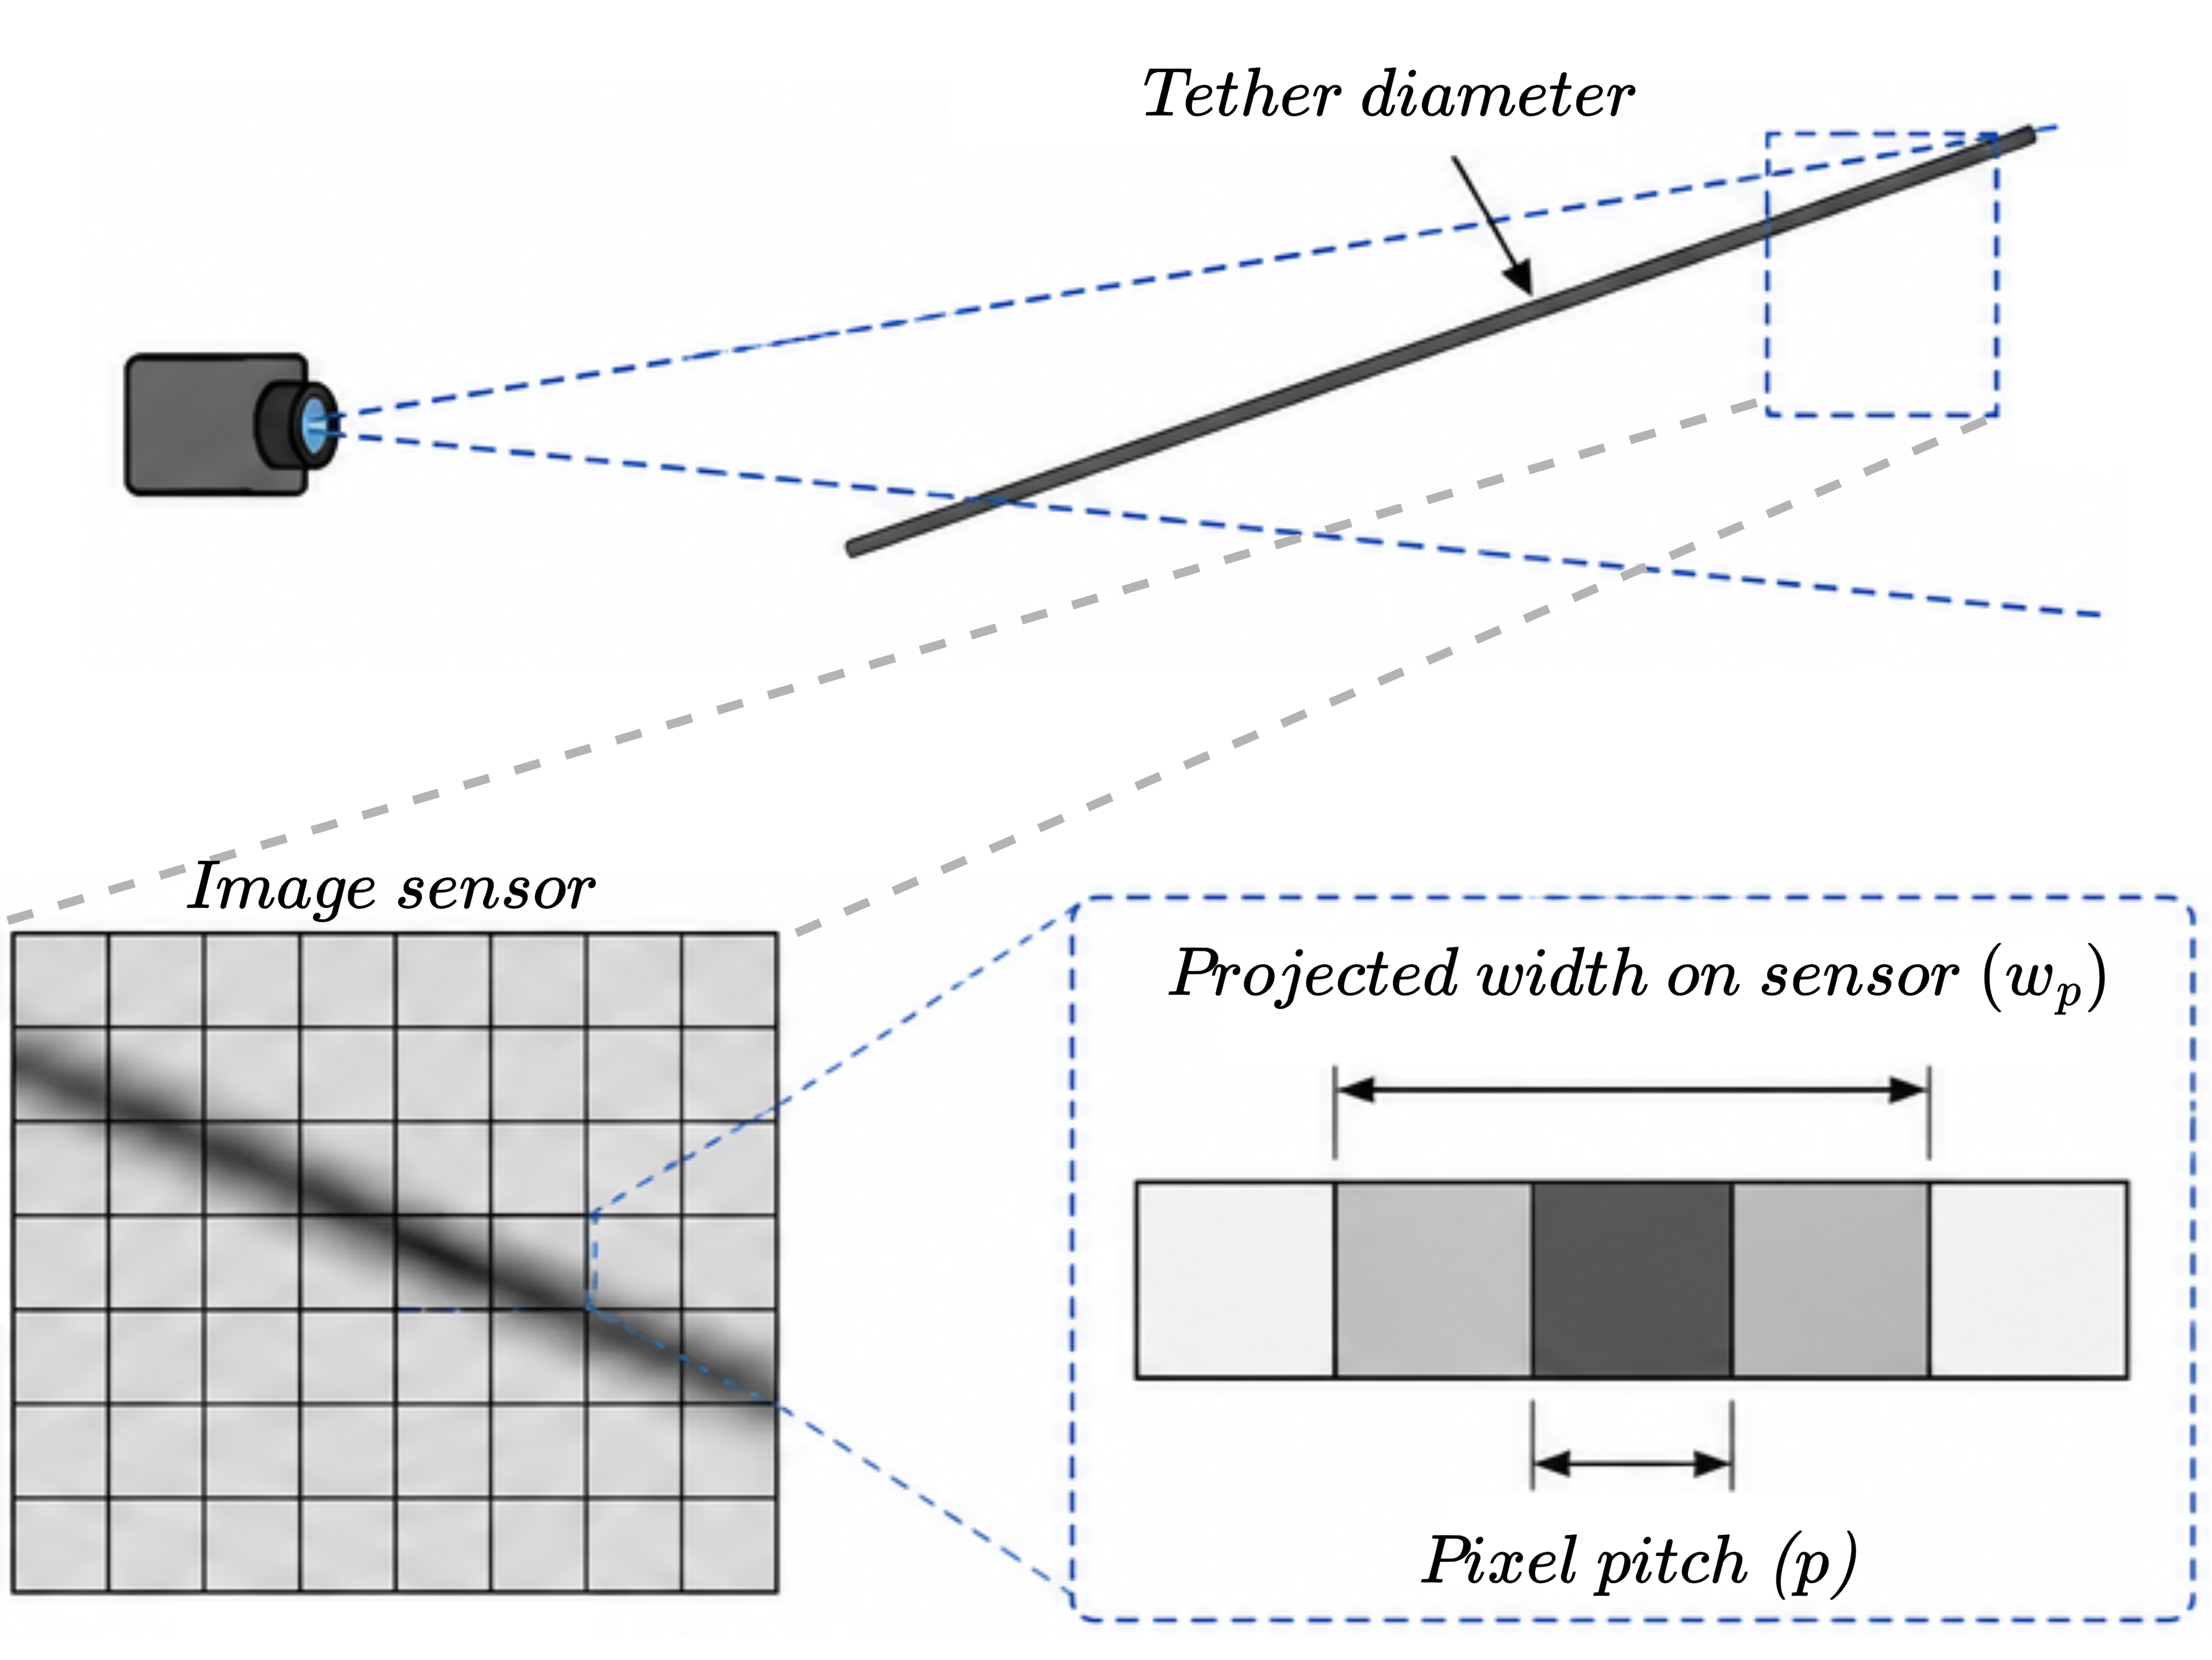
\includegraphics[width=0.8\textwidth]{PUCP_pictures/Stereo vision system/Figure1.5a.png}
    \caption{Projection of the tether cross-section onto the image sensor.}
    \label{fig:figure1.5a}
\end{figure}

\begin{figure}[H]
    \centering
    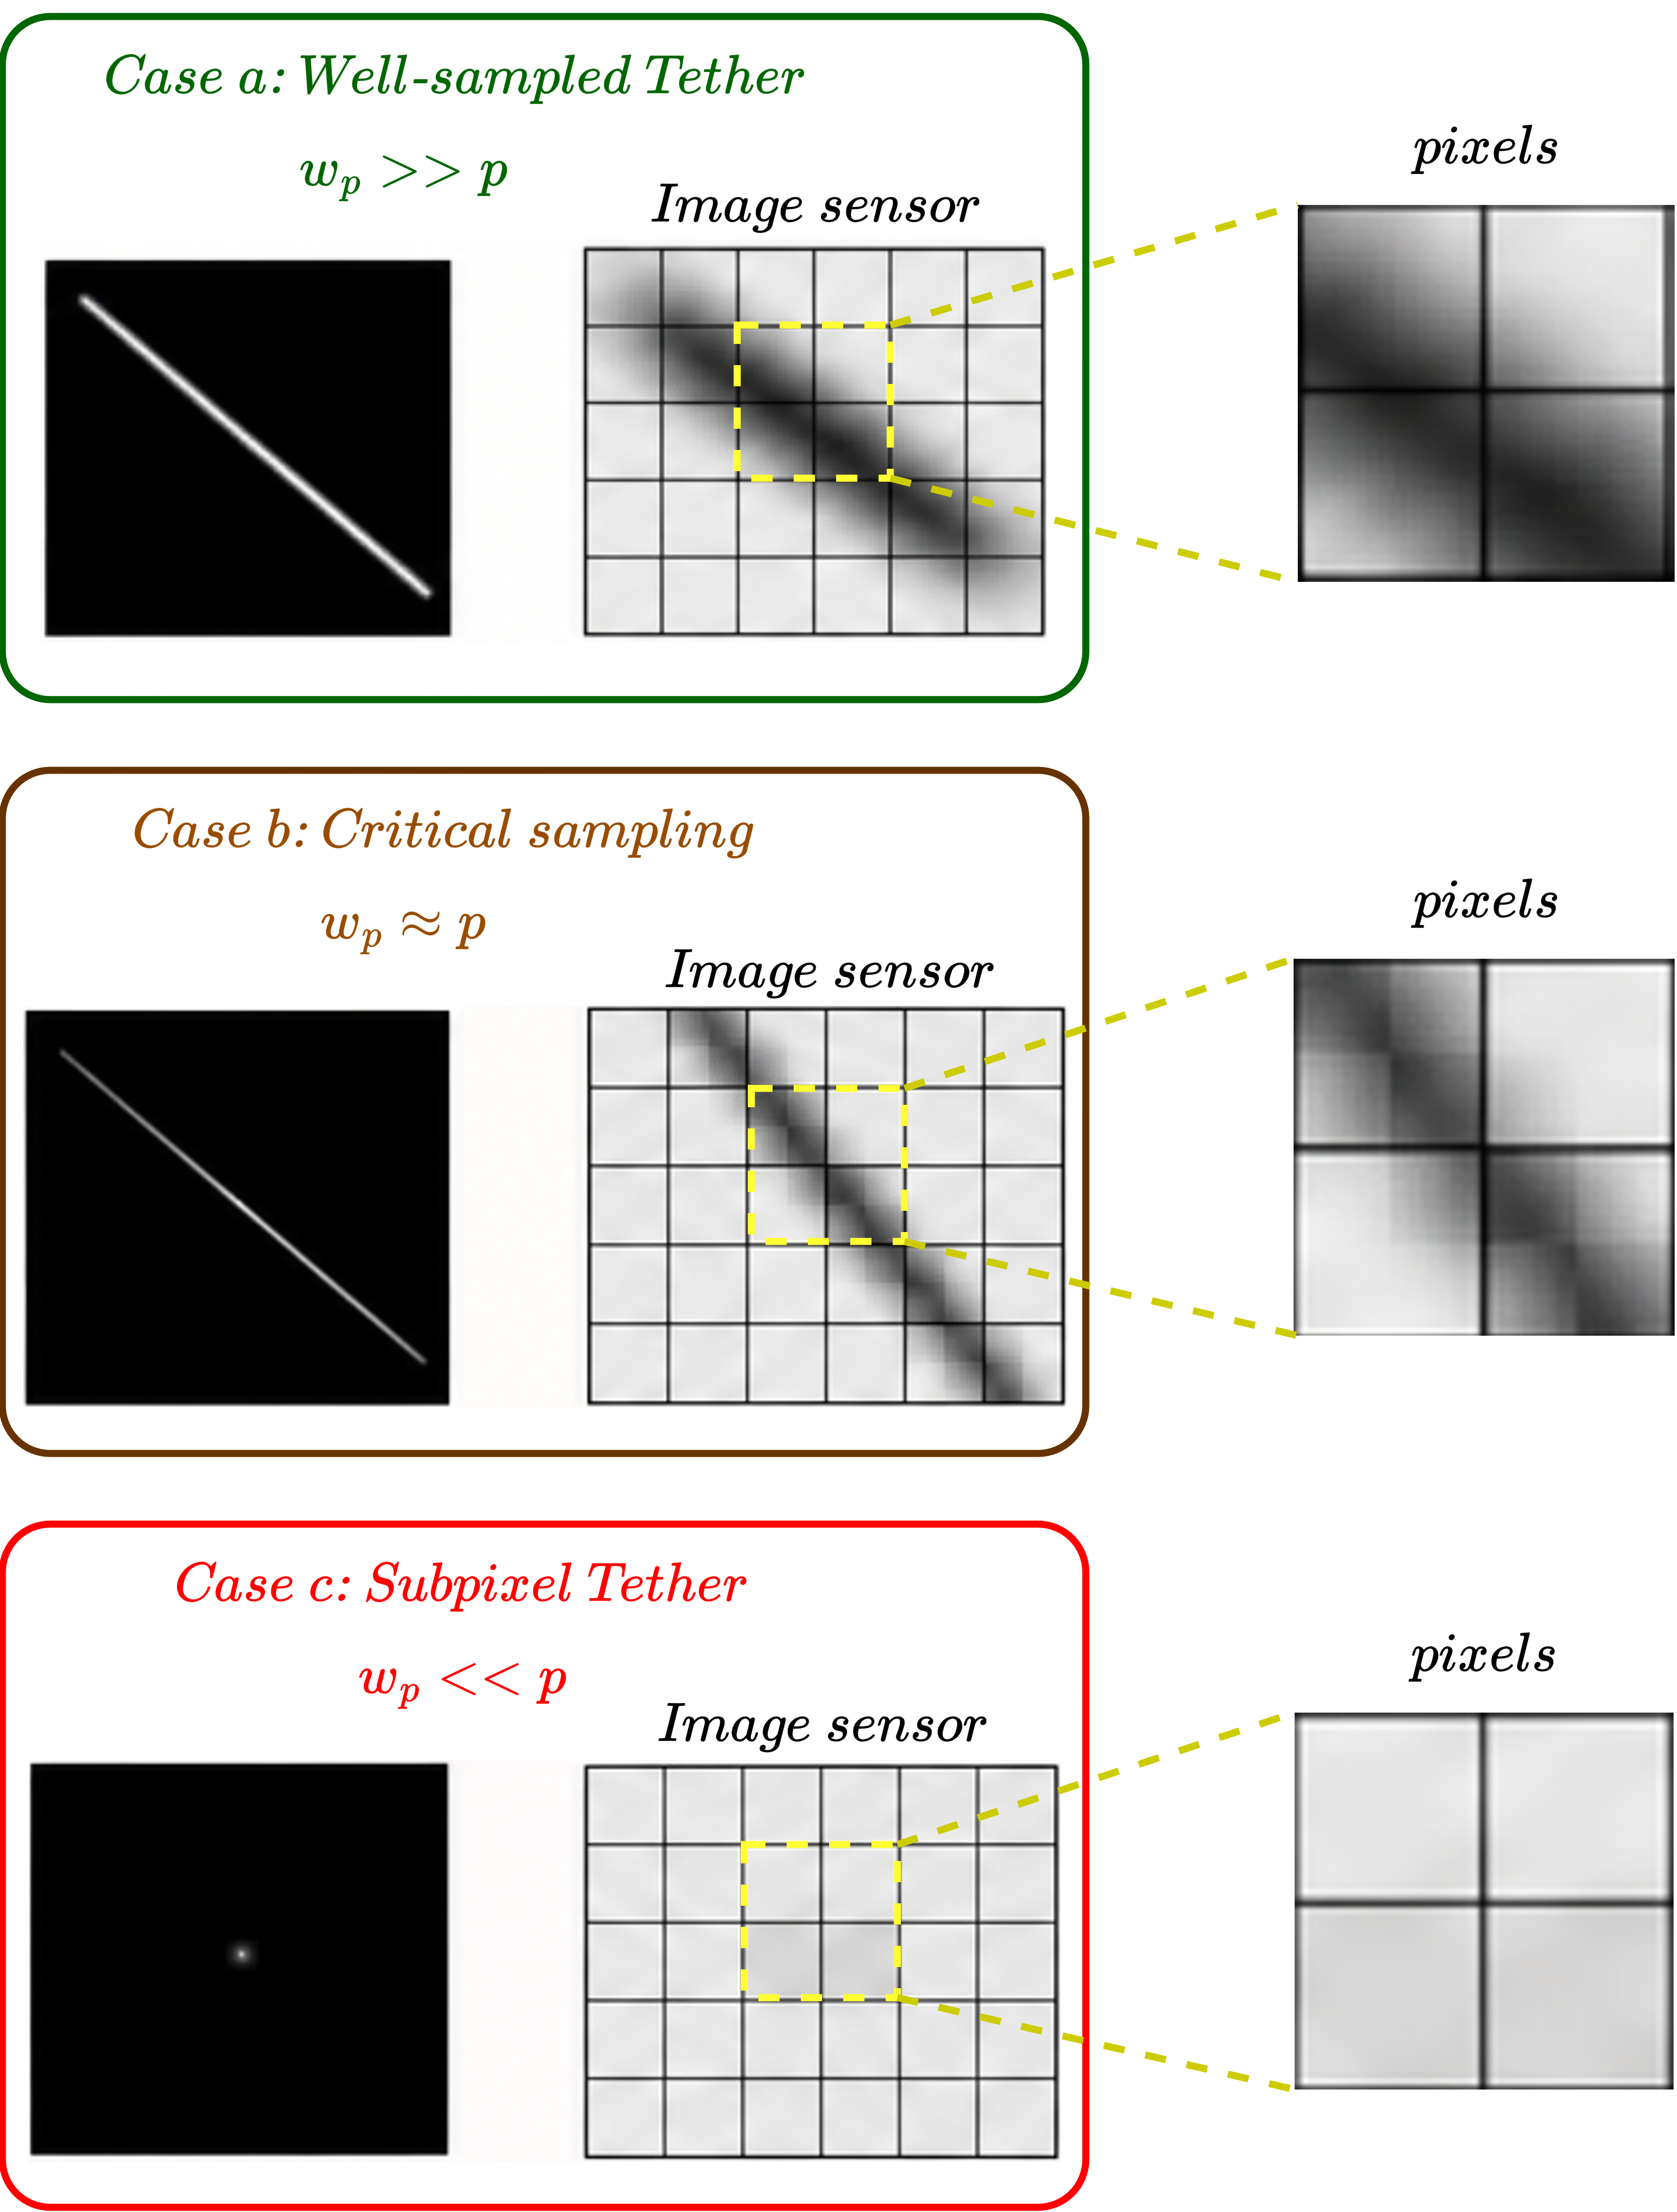
\includegraphics[width=0.75\textwidth]{PUCP_pictures/Stereo vision system/Figure1.5b.png}
    \caption{Geometric detectability regimes of the tether as a function of projected width and pixel pitch.}
    \label{fig:figure1.5b}
\end{figure}

In addition to geometric sampling, tether detectability is also affected by radiometric contrast, directional illumination, and temporal visibility. These effects determine whether the tether signal can be distinguished from the background, how its brightness changes with Sun--tether--observer geometry, and whether visibility remains continuous or intermittent during orbital operation.

\vspace{0.3cm}
\noindent\textbf{Conventional Photogrammetry Assessment}

Standard photogrammetric reconstruction methods were evaluated to determine whether conventional feature matching and dense stereo correspondence could reconstruct target geometry under low-texture conditions. The analysis considered two representative targets with different levels of reconstruction difficulty.

The first target was a volumetric object, represented by a bottle. This object was selected as a simple reference case because it occupies a significant number of pixels and contains a geometry that is generally compatible with conventional photogrammetric reconstruction when sufficient visual information is available. The second target was the tether proxy, which represents the main object of interest for the LINKU mission. Unlike the bottle, the tether is a thin and low-texture structure, making it significantly more difficult to reconstruct using conventional photogrammetry, even when environmental texture is available.

The first analysis reconstructed the bottle under a low-texture background condition, representative of the reduced visual references expected in orbital observation. When the background texture was reduced, dense stereo reconstruction yielded unstable disparity estimates and noisy three-dimensional outputs. After manual removal of disparity artifacts, the remaining reconstruction remained limited and incomplete, indicating that post-processing alone does not resolve the underlying dependence on reliable stereo correspondence.

The second analysis evaluated the tether proxy under a textured background condition. This configuration intentionally provided environmental visual features to facilitate image alignment and assess whether conventional Structure-from-Motion methods could recover the tether geometry when supported by background texture. The reconstruction demonstrated that environmental texture can support image alignment and partial scene reconstruction, as shown in Figure~\ref{fig:figure1.6}. However, this result also confirmed that the reconstruction was mainly supported by the surrounding environment rather than by the tether itself.

\begin{figure}[htbp]
    \centering
    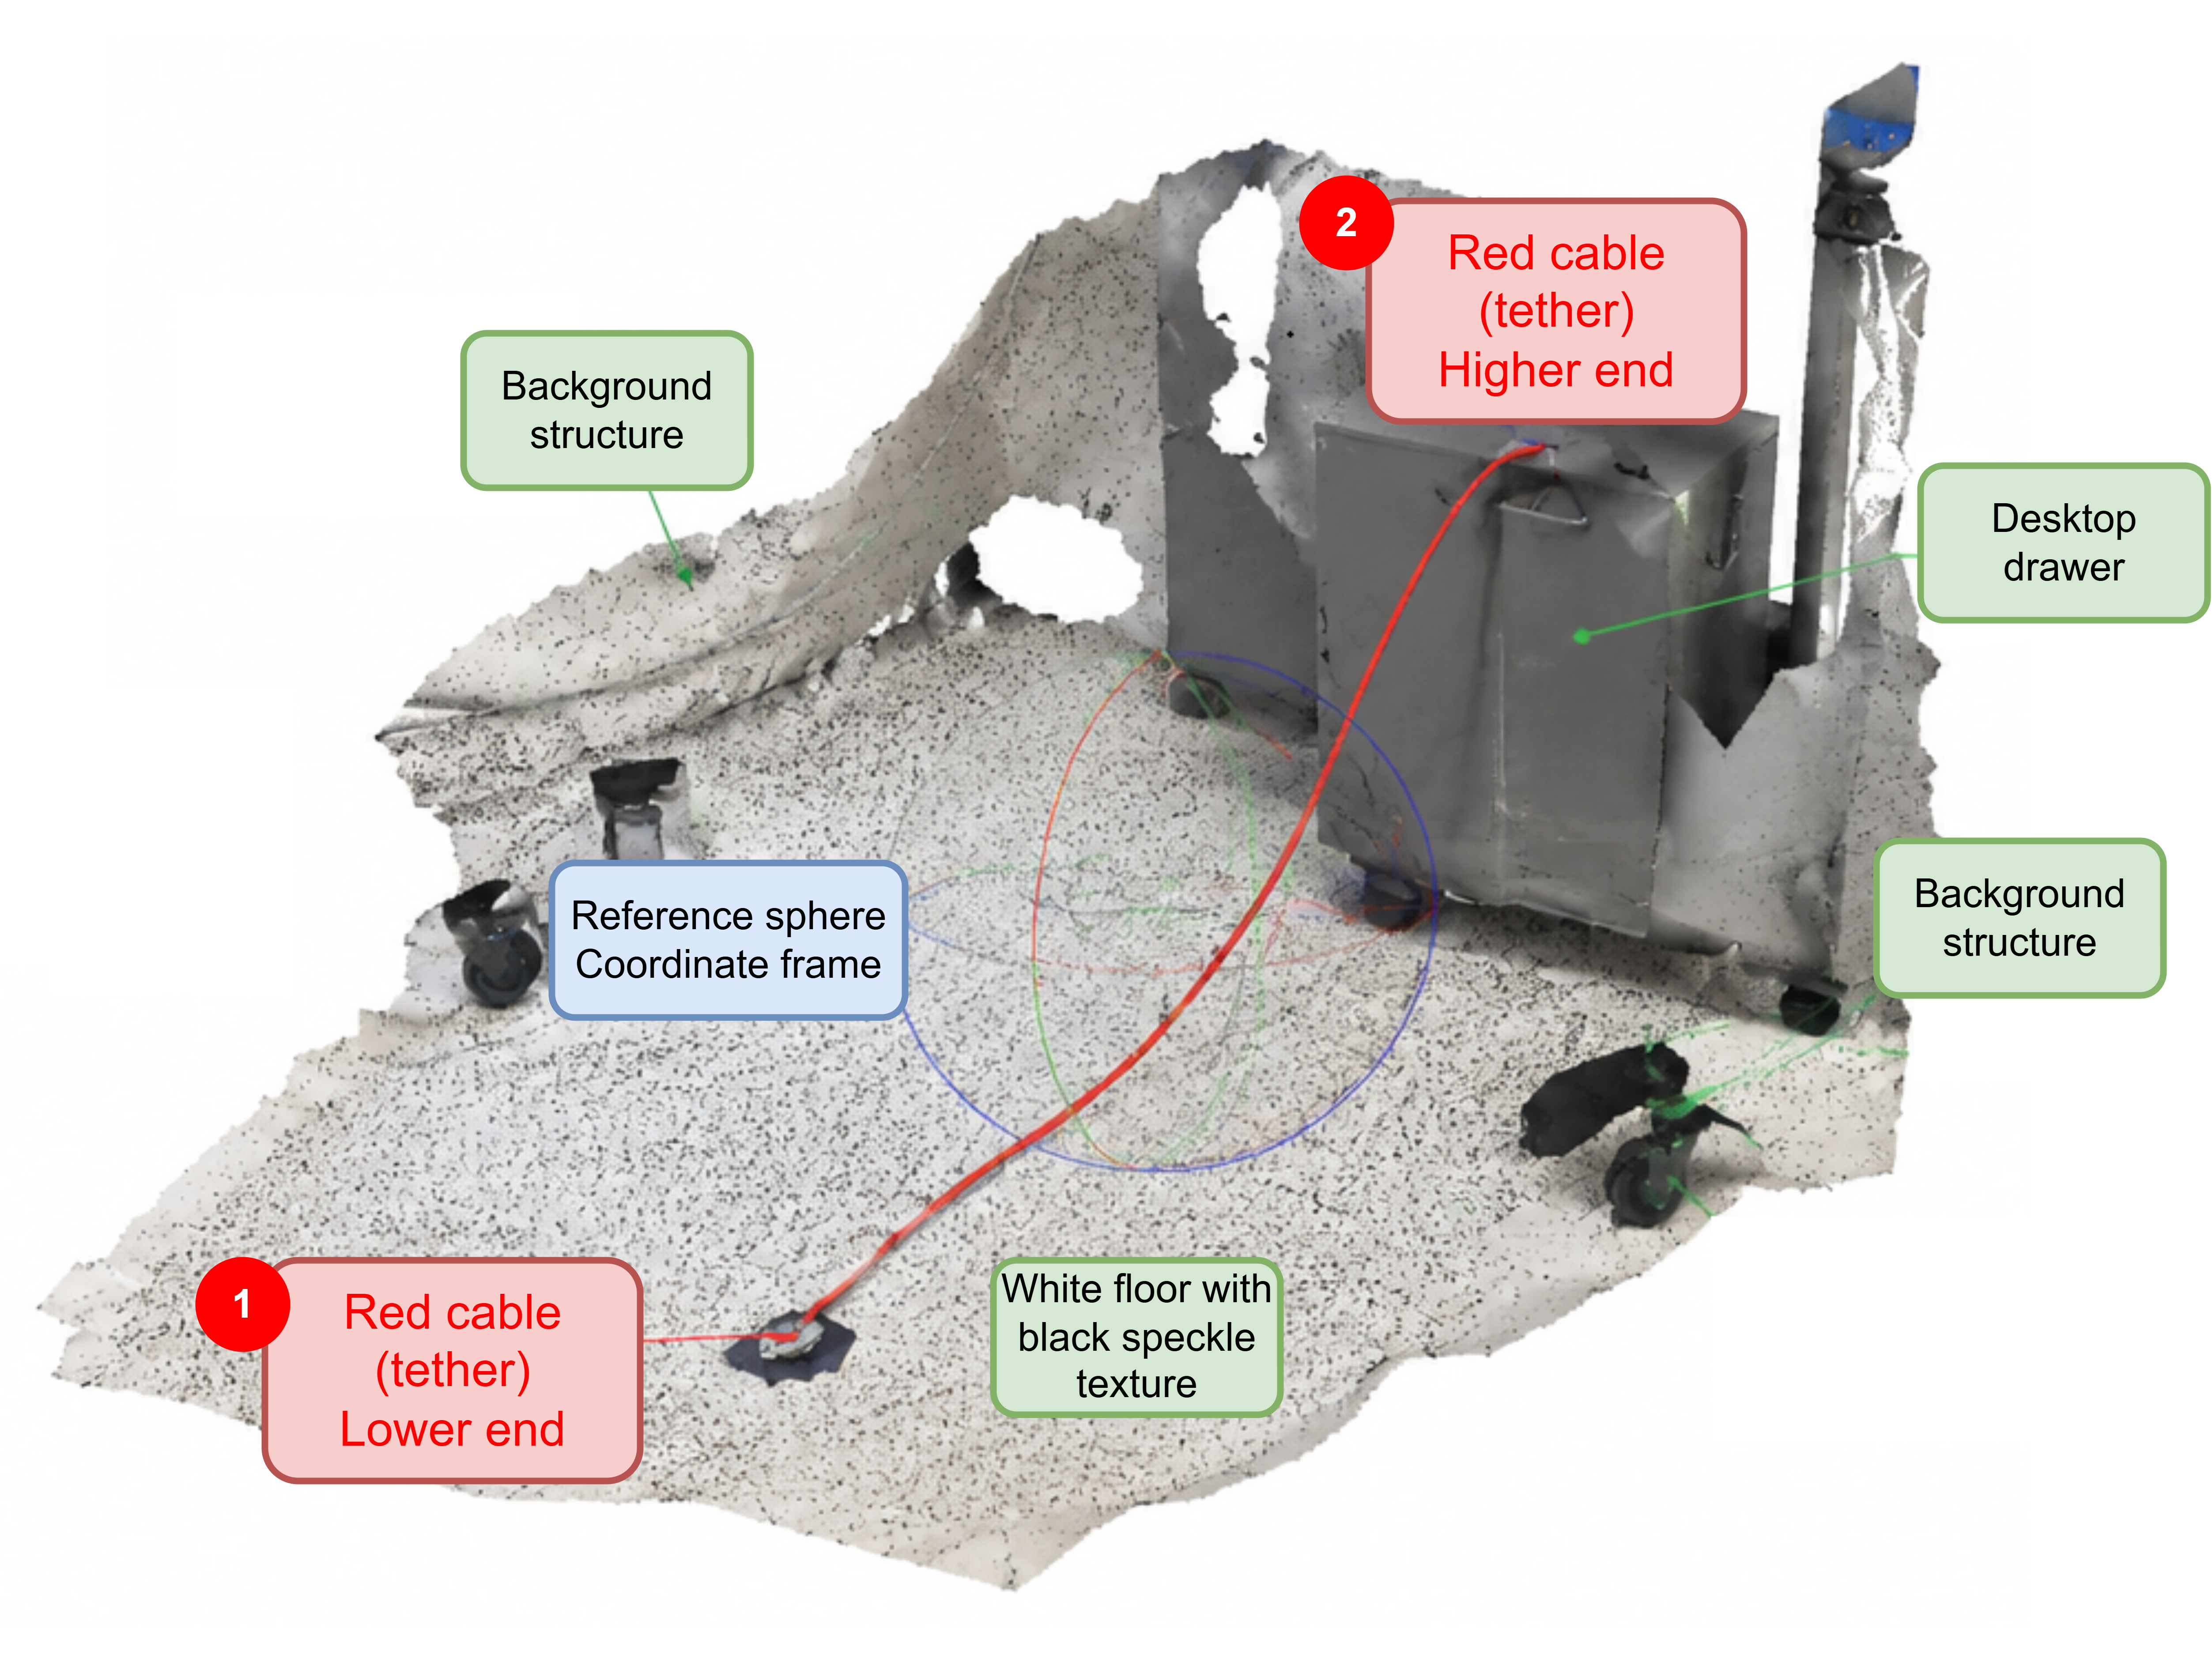
\includegraphics[width=\textwidth]{PUCP_pictures/Stereo vision system/Figure1.6.png}
    \caption{Structure-from-Motion reconstruction supported by environmental texture.}
    \label{fig:figure1.6}
\end{figure}

Finally, the tether was processed without the supporting background texture to evaluate its reconstruction under a more representative isolated observation condition. In this case, the reconstruction failed and produced a ``Zero Resolution'' condition, as shown in Figure~\ref{fig:figure1.7}. This result demonstrates that conventional photogrammetry is not suitable for isolated tether reconstruction under low-texture conditions.

Overall, these tests show that conventional photogrammetric methods are strongly dependent on environmental texture and stable visual features. While a volumetric object may still provide partial reconstruction information under constrained conditions, the tether proxy does not provide sufficient texture or geometric support for reliable conventional reconstruction. This finding motivates the use of the geometry-driven reconstruction methodology evaluated in the following section.

\begin{figure}[H]
    \centering
    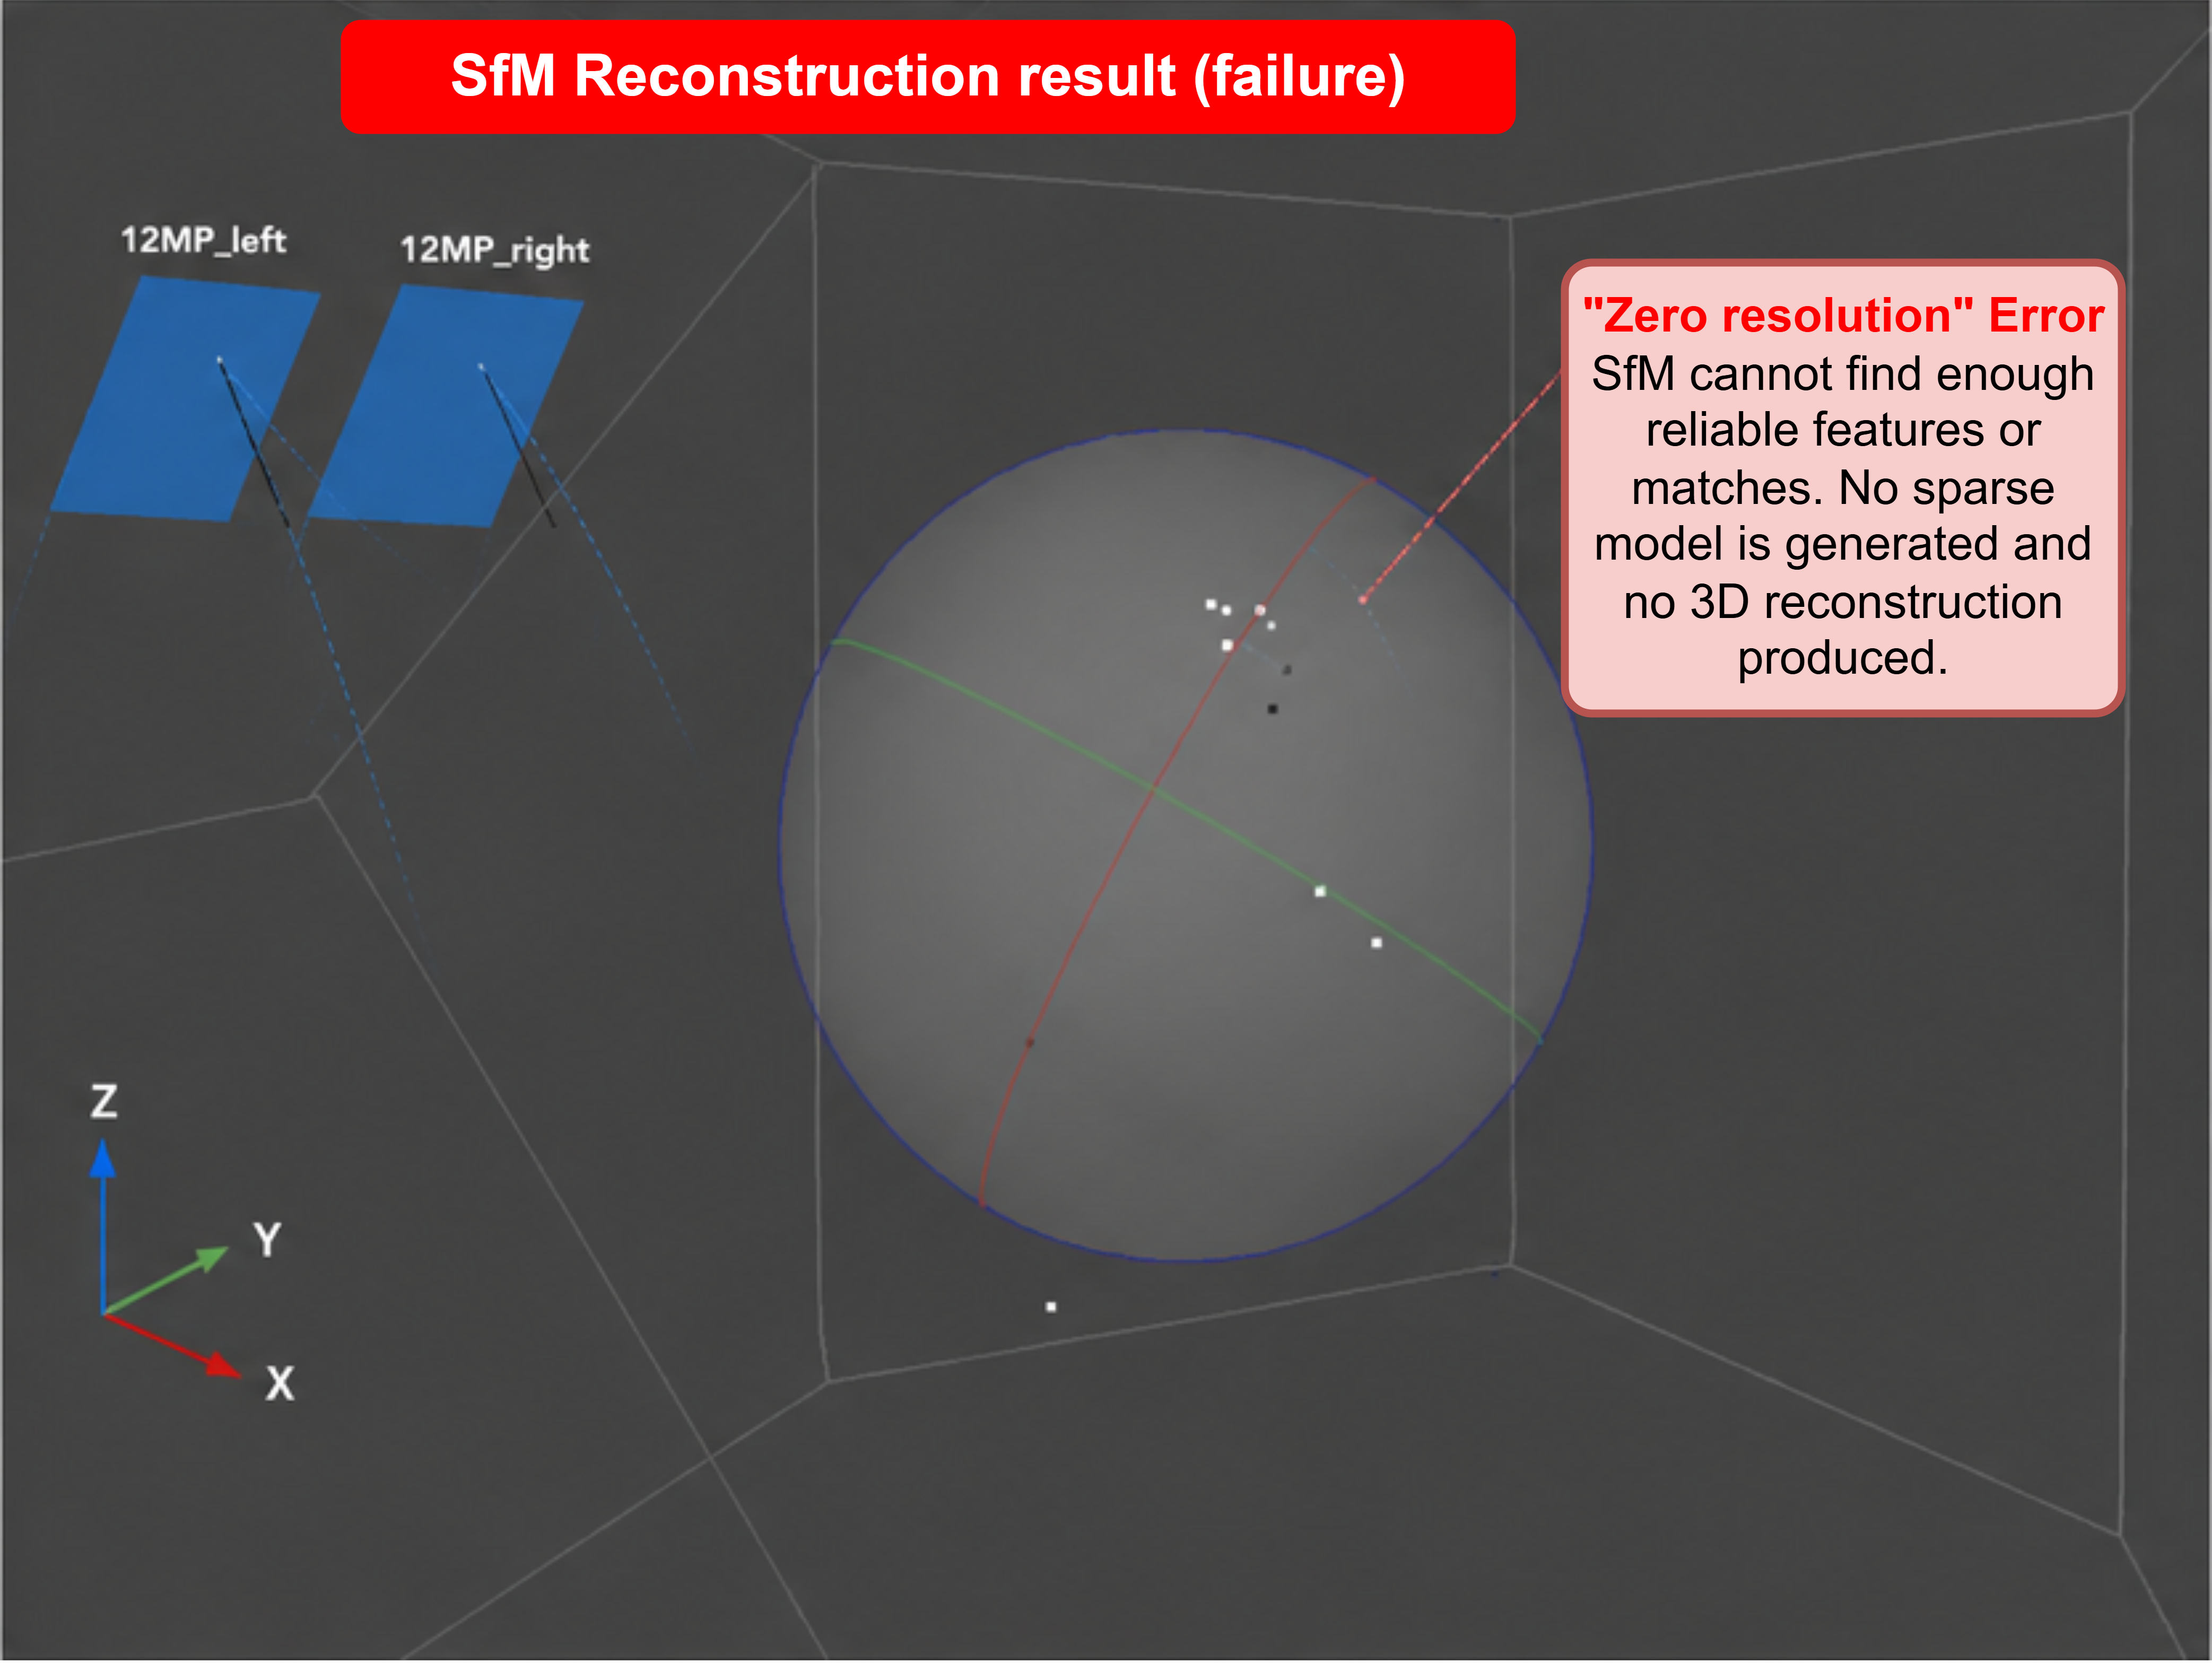
\includegraphics[width=\textwidth]{PUCP_pictures/Stereo vision system/Figure1.7.png}
    \caption{Tether-only reconstruction attempt after background removal, resulting in a ``Zero Resolution'' failure.}
    \label{fig:figure1.7}
\end{figure}

\newpage
\vspace{0.3cm}
\noindent\textbf{Geometry-Driven Reconstruction Tests}

The primary experimental validation focused on the proposed geometry-driven reconstruction method. Two tether configurations were evaluated. Scenario A corresponded to a predominantly planar tether configuration with limited depth variation, while Scenario B introduced stronger out-of-plane deformation and depth variation, as shown in Figures~\ref{fig:figureplanar} and~\ref{fig:figure3d}.

\begin{figure}[htbp]
    \centering
    \begin{subfigure}{\textwidth}
        \centering
        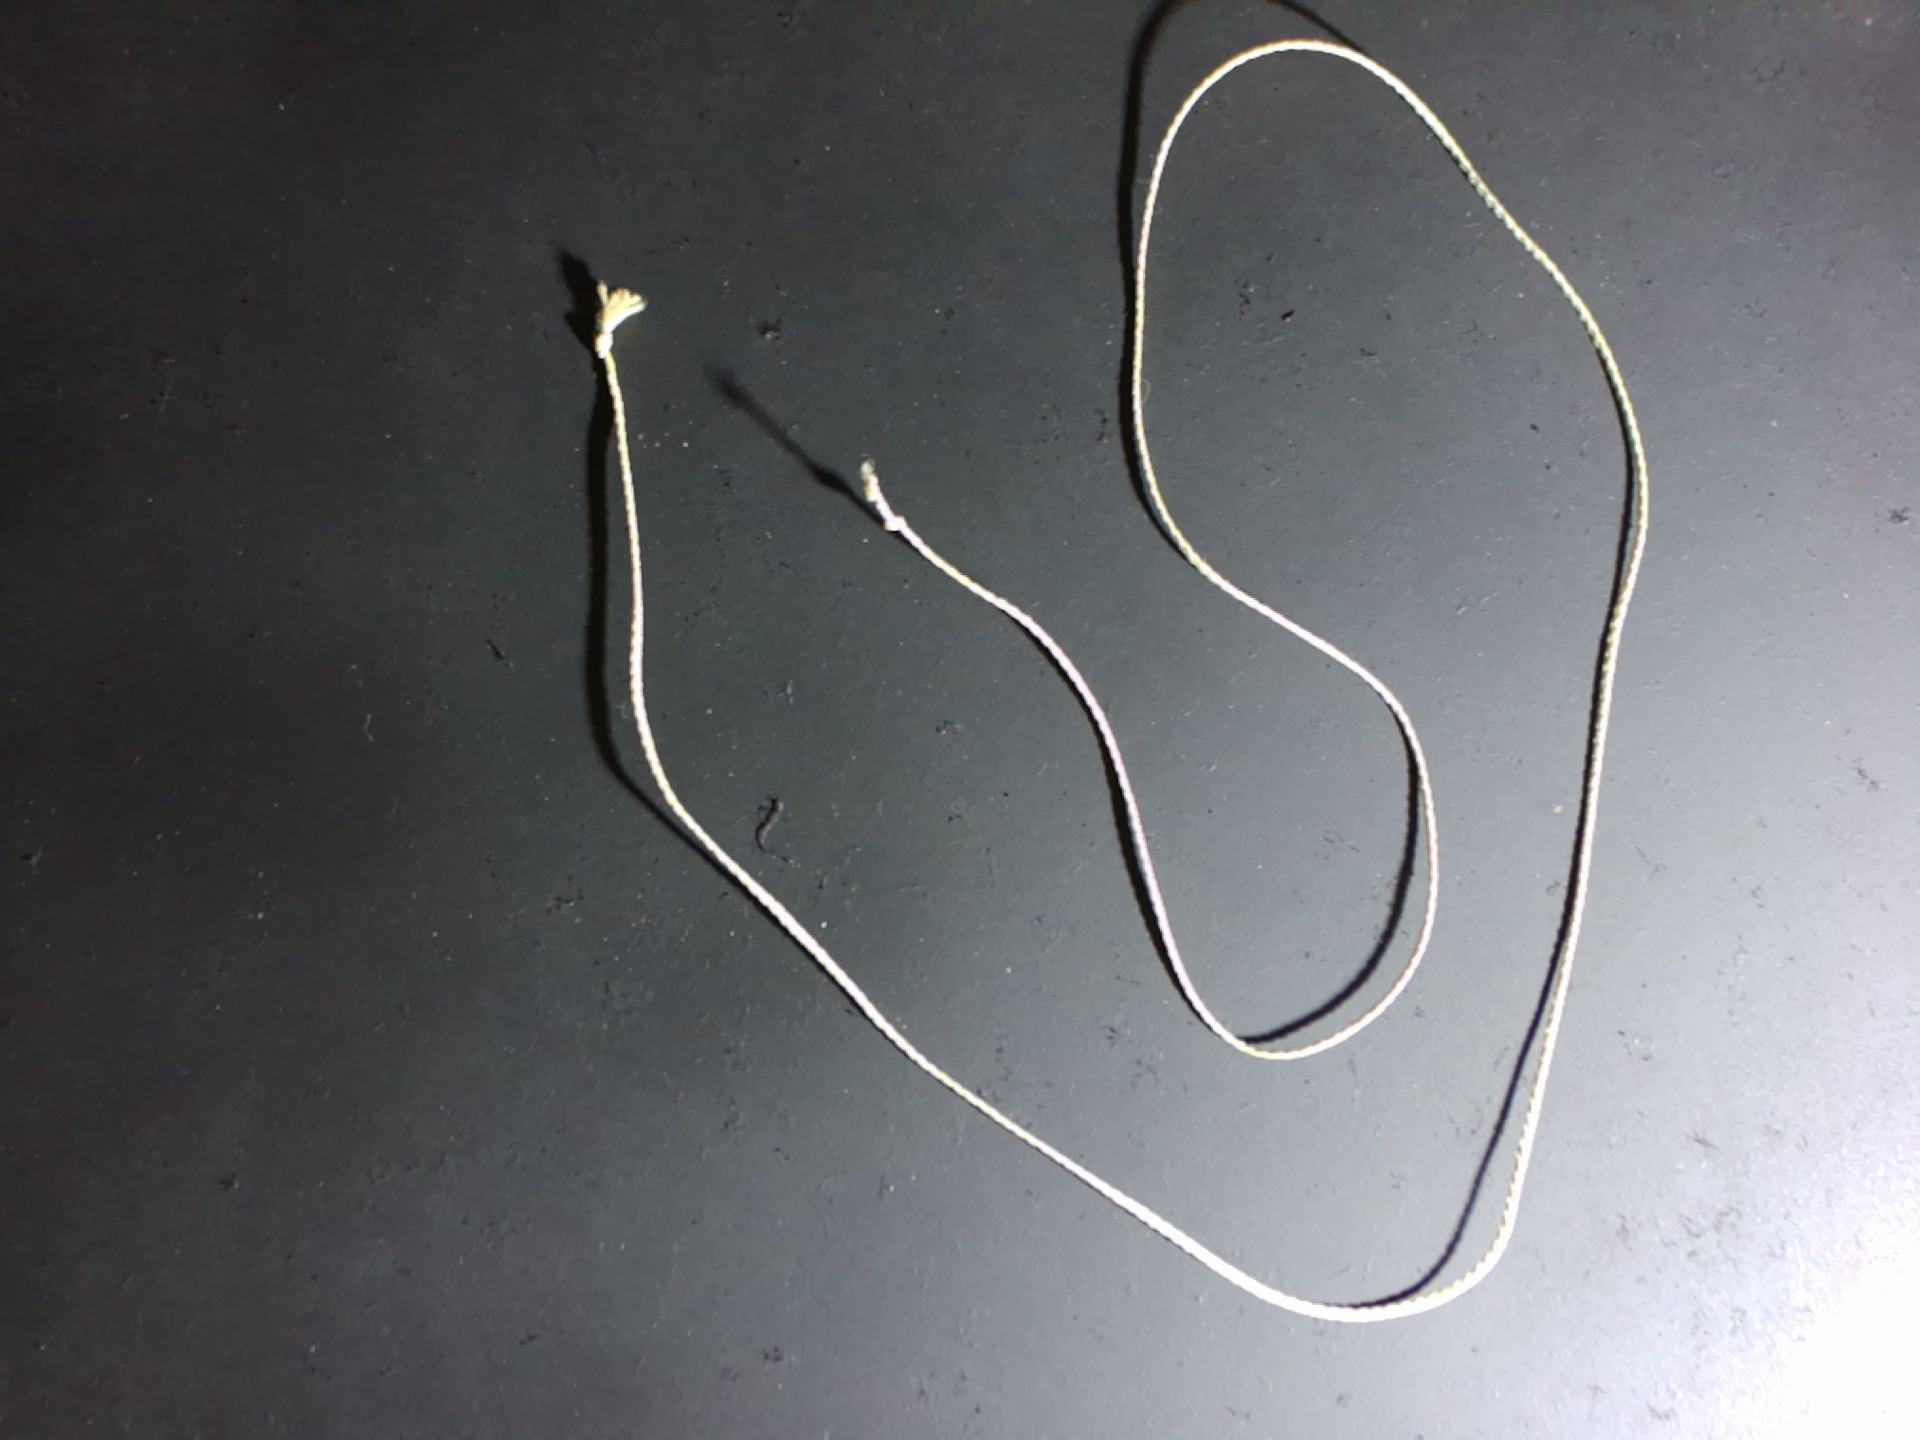
\includegraphics[
            height=7cm,
            keepaspectratio
        ]{PUCP_pictures/Stereo vision system/Figureplanar.jpg}
        \caption{}
        \label{fig:figureplanar}
    \end{subfigure}
    \vspace{0.4cm}
    \begin{subfigure}{\textwidth}
        \centering
        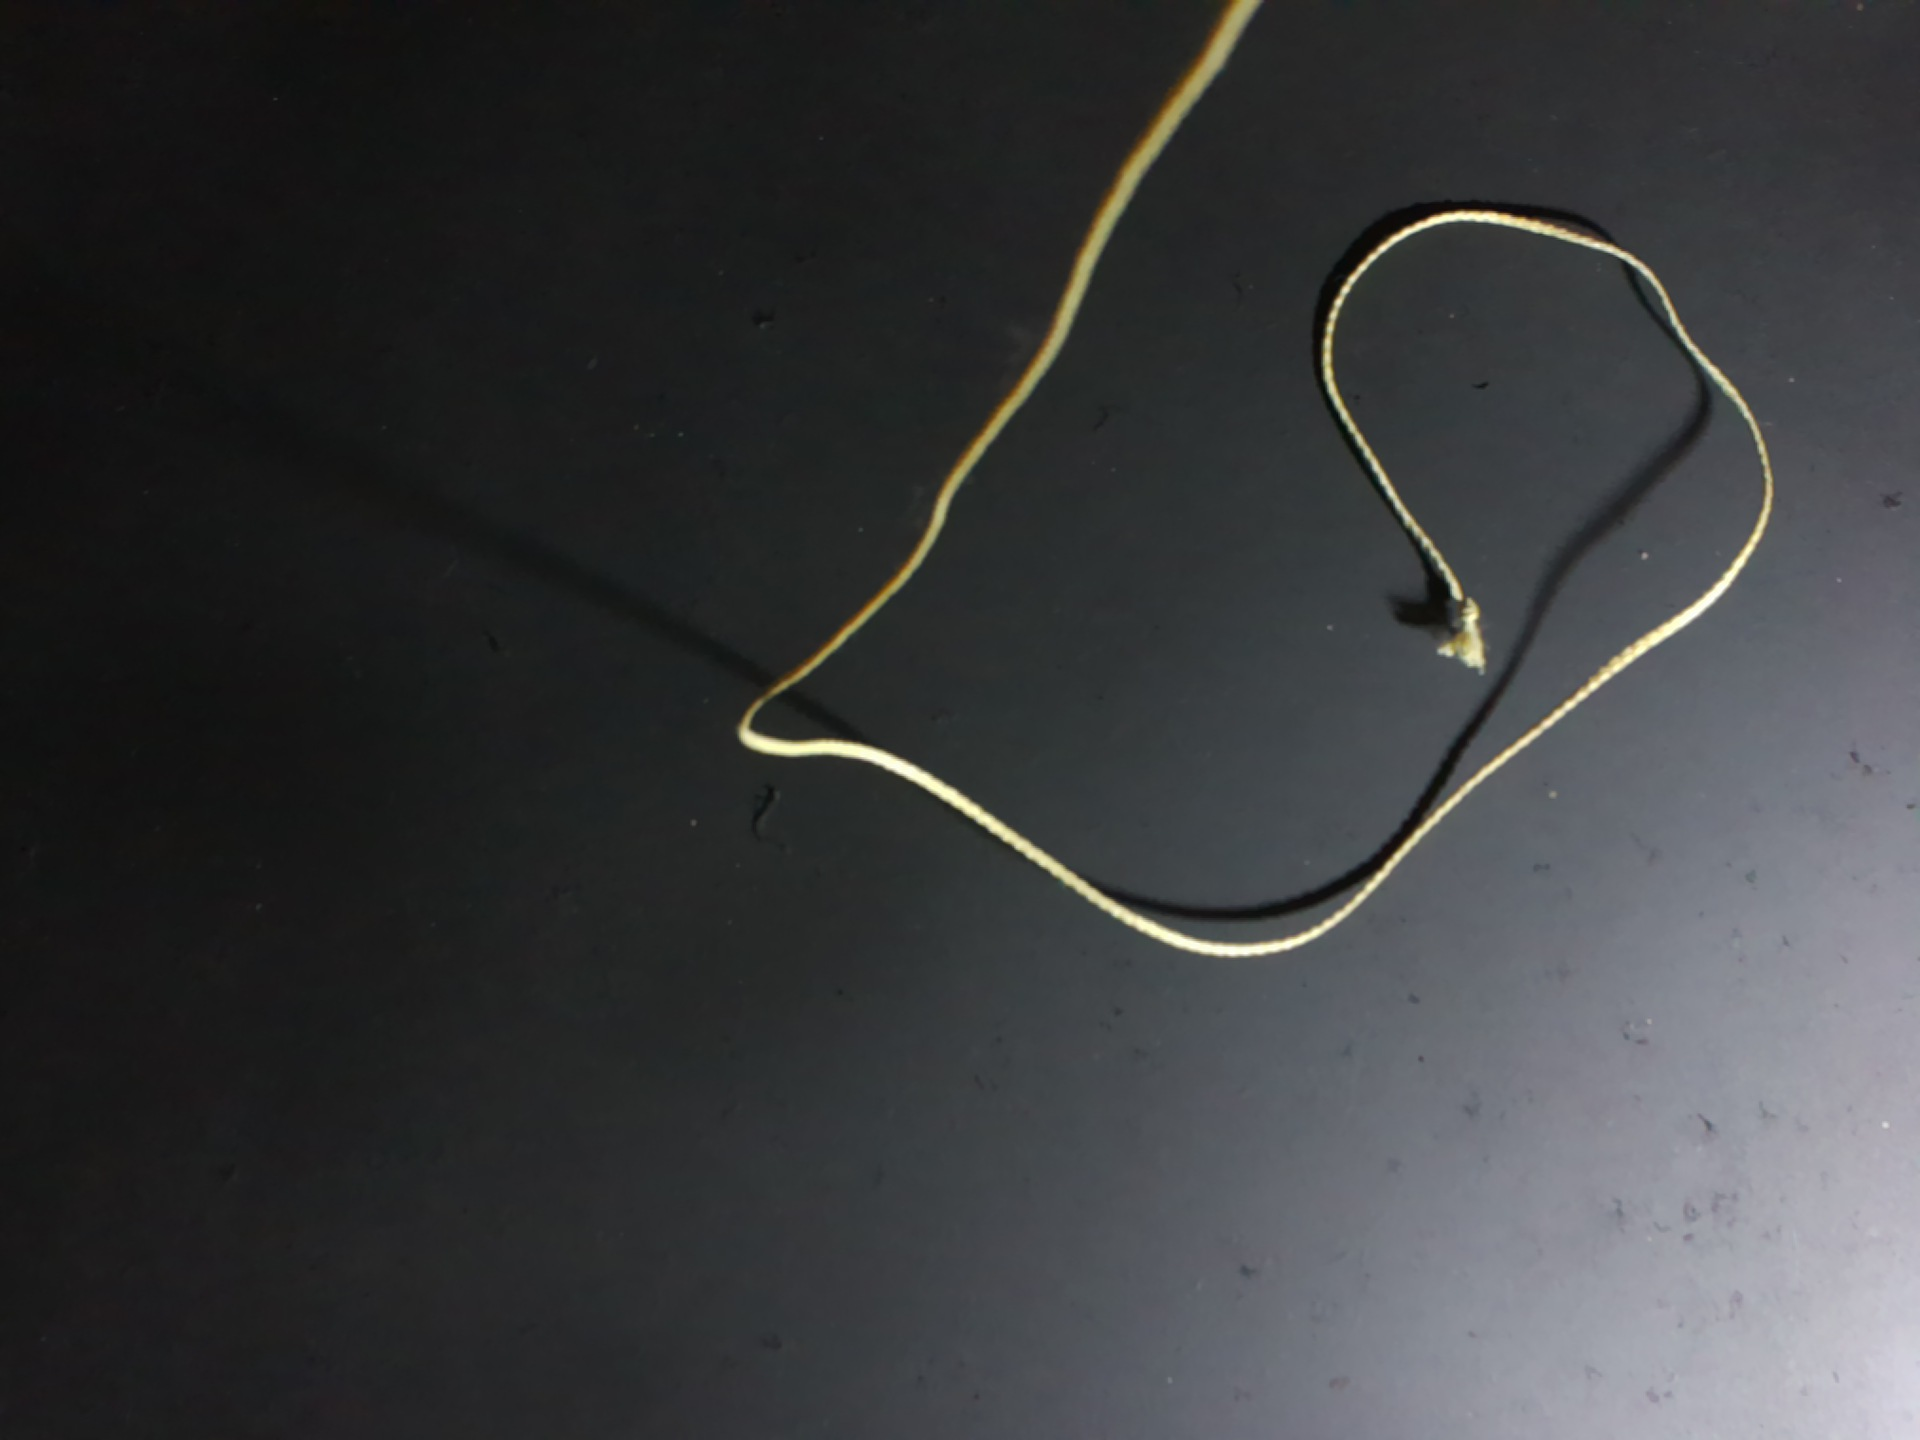
\includegraphics[
            height=7cm,
            keepaspectratio
        ]{PUCP_pictures/Stereo vision system/Figure3d.jpg}
        \caption{}
        \label{fig:figure3d}
    \end{subfigure}
    \caption{Experimental scenarios for geometry-driven tether reconstruction:
    (a) Scenario A, planar tether configuration;
    (b) Scenario B, out-of-plane tether configuration.}
    \label{fig:scenarios}
\end{figure}

The process begins with the simultaneous acquisition of left and right images using a calibrated stereo camera configuration. The tether is then isolated in both views and reduced to a one-pixel-wide centerline, which serves as the geometric representation for correspondence estimation. Next, epipolar constraints are applied to identify matched points along the extracted centerlines. Each corresponding point pair is subsequently triangulated to estimate its 3D position. Finally, the reconstructed point set is visualized in three-dimensional space to recover the tether spatial configuration.

Figures~\ref{fig:figure2.0} and~\ref{fig:figure2.1} present the complete geometry-driven workflow, from stereo image acquisition to three-dimensional tether representation, for Scenarios A and B.

\begin{landscape}
\begin{figure}[htbp]
    \centering
    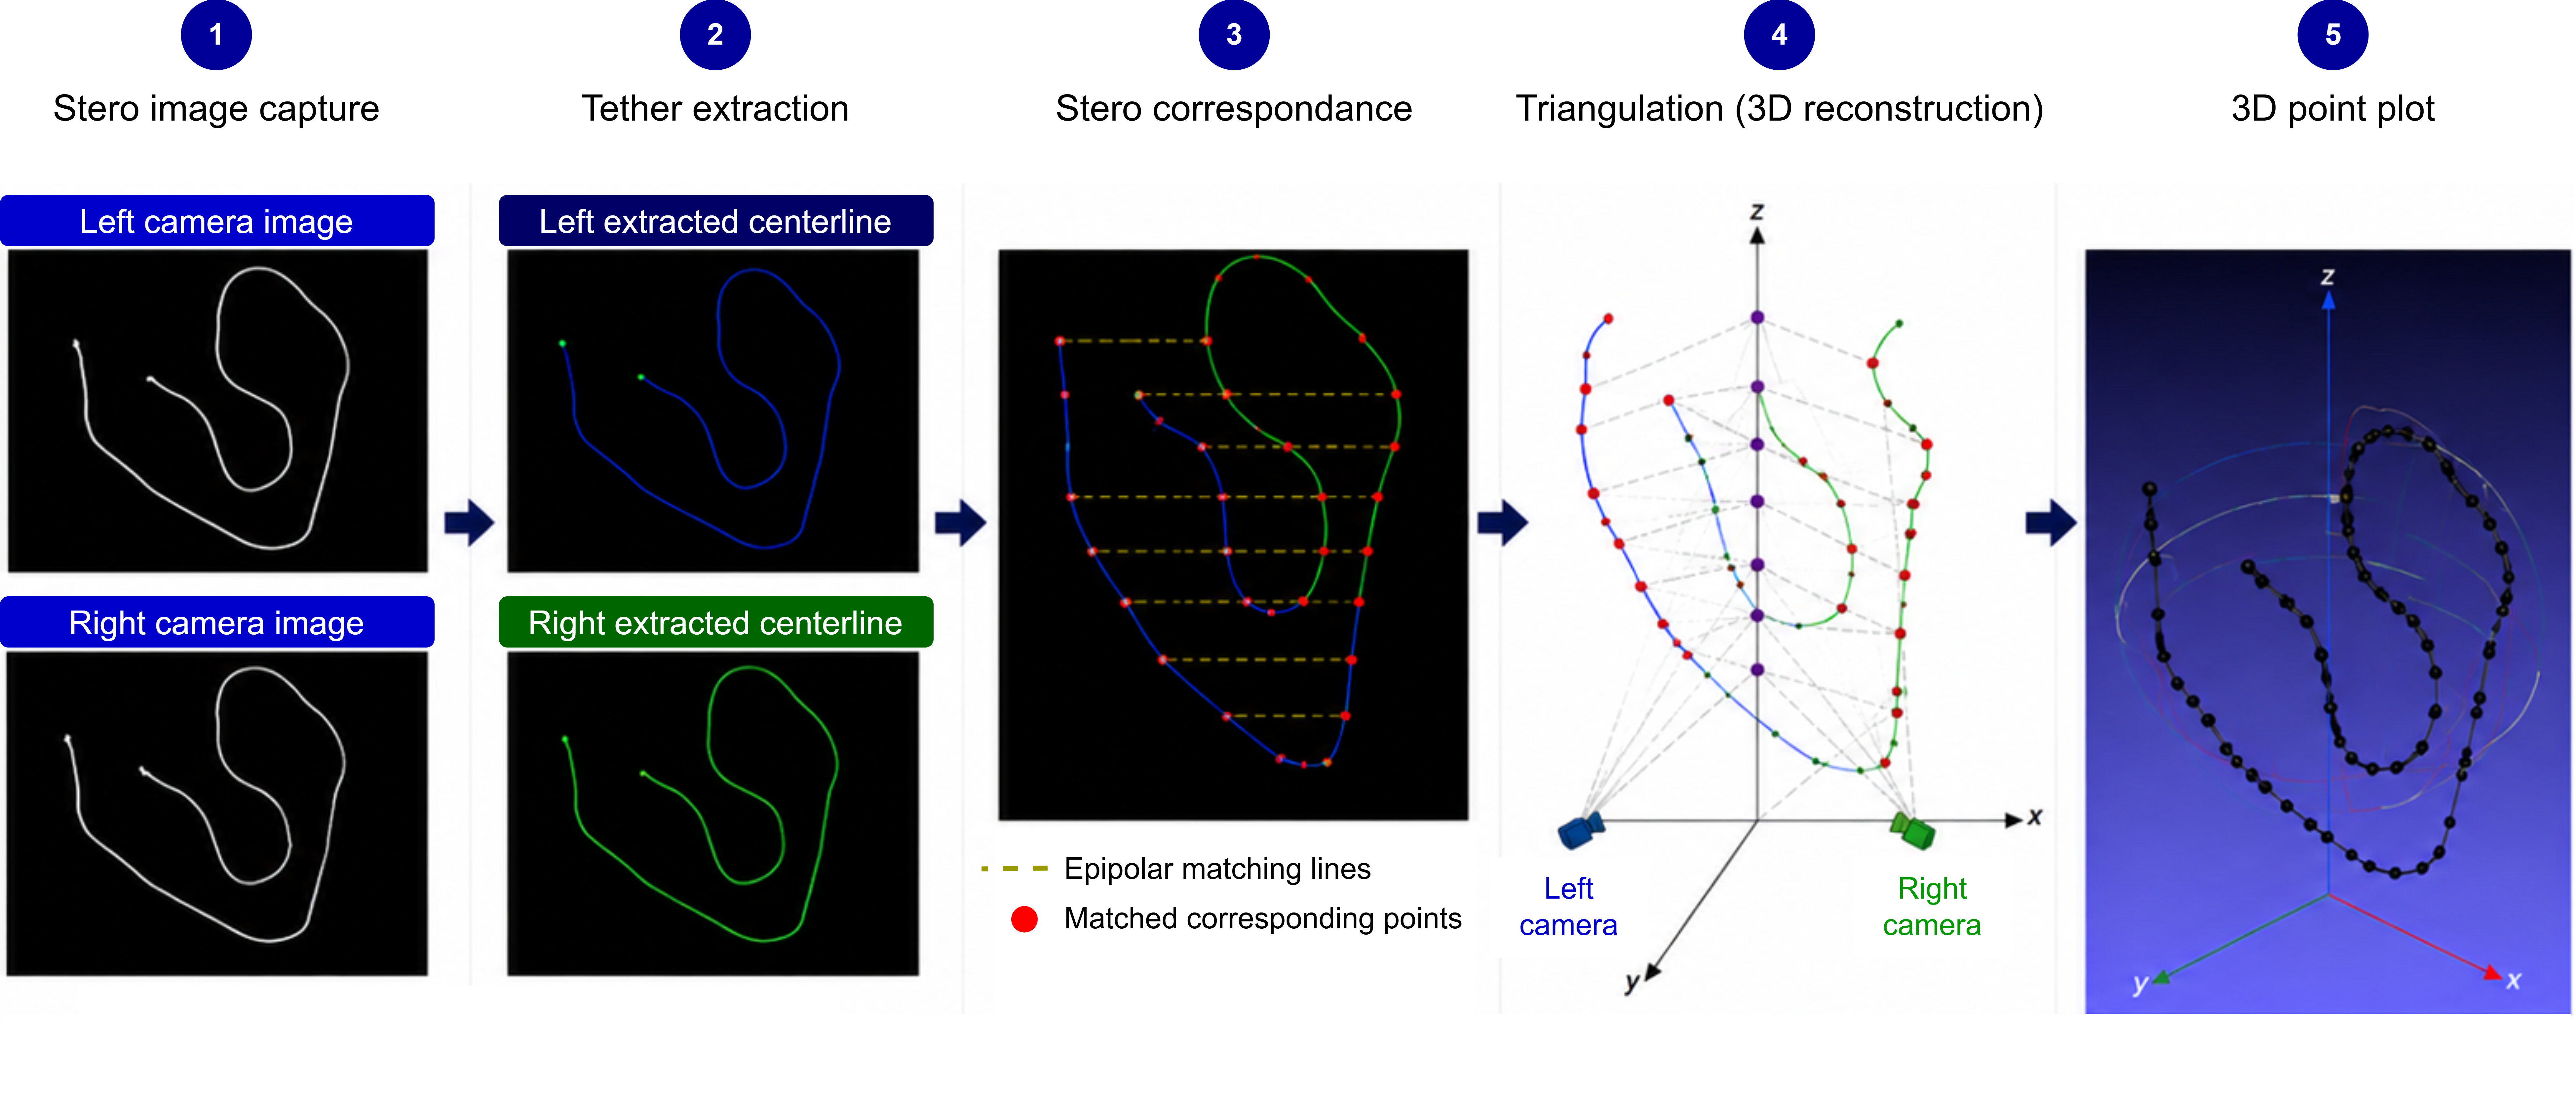
\includegraphics[width=1.75\textwidth]{PUCP_pictures/Stereo vision system/Figure2.0.png}
    \caption{Geometry-driven stereo reconstruction workflow for Scenario A.}
    \label{fig:figure2.0}
\end{figure}
\end{landscape}

\begin{landscape}
\begin{figure}[htbp]
    \centering
    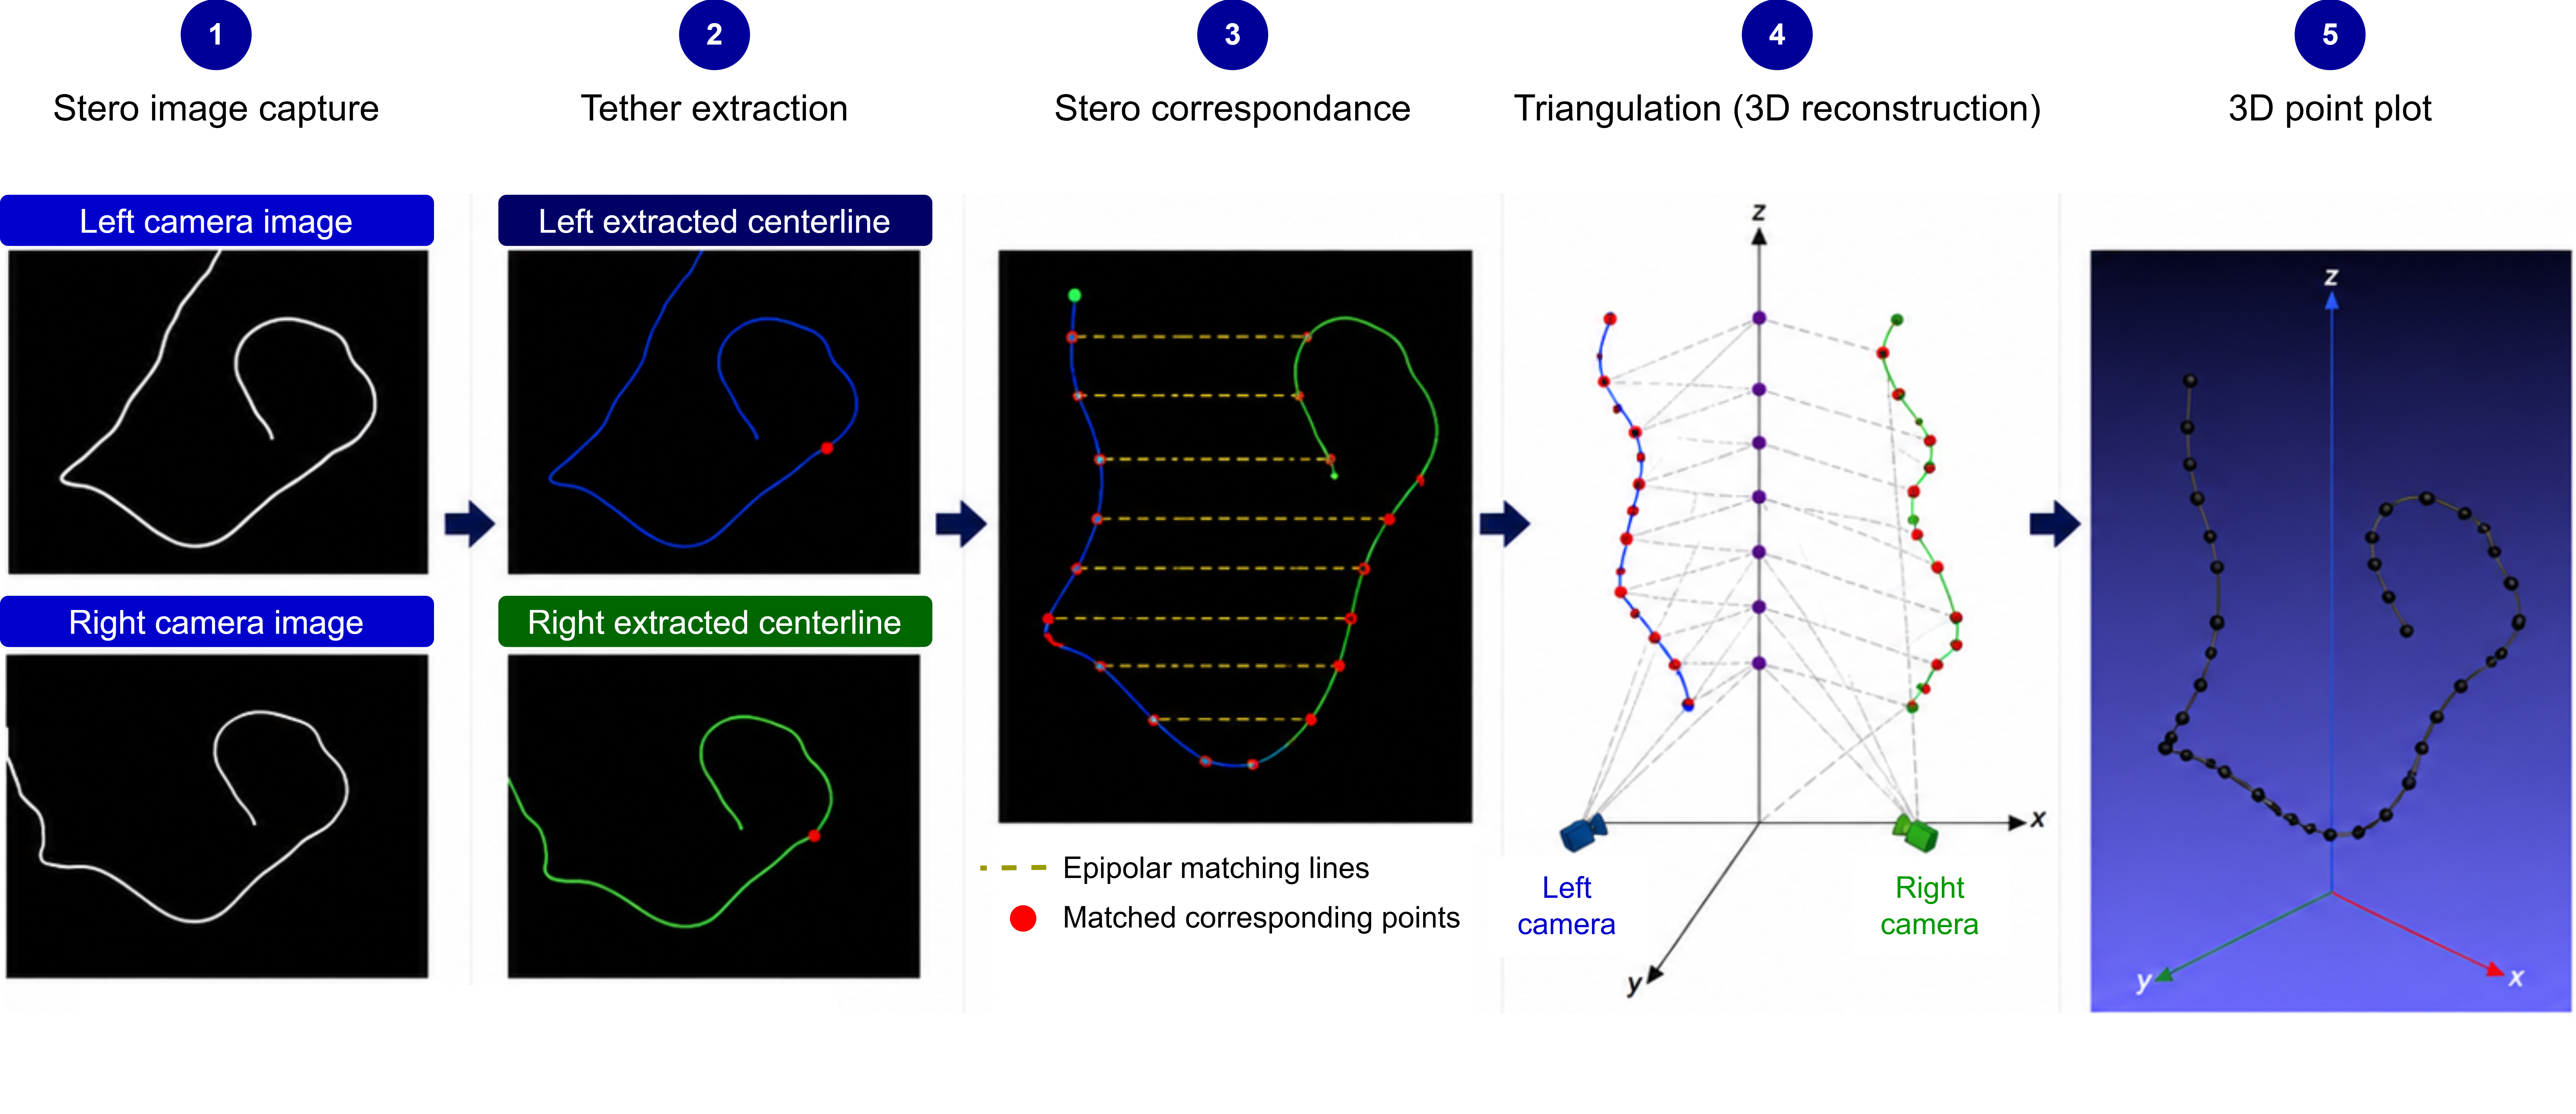
\includegraphics[width=1.75\textwidth]{PUCP_pictures/Stereo vision system/Figure2.1.png}
    \caption{Geometry-driven stereo reconstruction workflow for Scenario B.}
    \label{fig:figure2.1}
\end{figure}
\end{landscape}

These results demonstrate that the geometry-driven reconstruction framework can recover continuous tether geometry under both planar and volumetric configurations, without relying on background texture, sparse visual features, or standard photogrammetric matching.

\subsubsection{Main Results Obtained}
\label{subsub:stereo_vision_main_results}

The principal results of the current work can be summarized as follows:

\begin{itemize}
    \item Conventional photogrammetry is not suitable as the primary reconstruction strategy for isolated tether observation under low-texture conditions. Its dependence on stable background texture and feature-rich scenes makes it unreliable for thin tether-like structures.
    \item The optical analysis confirmed that a millimeter-scale tether enters the sub-pixel regime at long observation distances. Increasing sensor resolution improves pixel occupancy but does not eliminate the need for radiometric detection and geometry-driven processing.
    \item The geometry-driven reconstruction framework successfully reconstructed continuous tether geometries under both planar and volumetric experimental configurations.
    \item The proposed method demonstrated that tether reconstruction can be achieved without relying on environmental texture, sparse visual features, or conventional feature-based matching.
    \item Topological crossings and self-intersections remain important challenges for future development. These cases require additional support from temporal tracking, topological reasoning, or targeted AI-assisted methods.
    \item AI-assisted approaches are more appropriate as complementary tools than as primary scientific reconstruction methods. Their most promising future roles include robust mask generation, knot solving, ambiguity resolution, and anomaly detection.
    \item The experimental results support the central premise of the current work: tether observation should be treated primarily as a geometric and radiometric reconstruction problem, not as a conventional texture-based photogrammetry problem.
\end{itemize}